%  LaTeX support: latex@mdpi.com
%  In case you need support, please attach all files that are necessary for compiling as well as the log file, and specify the details of your LaTeX setup (which operating system and LaTeX version / tools you are using).

%=================================================================
\documentclass[water,article,submit,moreauthors,pdftex]{mdpi}

% If you would like to post an early version of this manuscript as a preprint, you may use preprint as the journal and change 'submit' to 'accept'. The document class line would be, e.g., \documentclass[preprints,article,accept,moreauthors,pdftex]{mdpi}. This is especially recommended for submission to arXiv, where line numbers should be removed before posting. For preprints.org, the editorial staff will make this change immediately prior to posting.

%% Some pieces required from the pandoc template
\providecommand{\tightlist}{%
  \setlength{\itemsep}{0pt}\setlength{\parskip}{4pt}}
\setlist[itemize]{leftmargin=*,labelsep=5.8mm}
\setlist[enumerate]{leftmargin=*,labelsep=4.9mm}

\usepackage{longtable}

% see https://stackoverflow.com/a/47122900

%--------------------
% Class Options:
%--------------------
%----------
% journal
%----------
% Choose between the following MDPI journals:
% acoustics, actuators, addictions, admsci, aerospace, agriculture, agriengineering, agronomy, algorithms, animals, antibiotics, antibodies, antioxidants, applsci, arts, asc, asi, atmosphere, atoms, axioms, batteries, bdcc, behavsci , beverages, bioengineering, biology, biomedicines, biomimetics, biomolecules, biosensors, brainsci , buildings, cancers, carbon , catalysts, cells, ceramics, challenges, chemengineering, chemistry, chemosensors, children, cleantechnol, climate, clockssleep, cmd, coatings, colloids, computation, computers, condensedmatter, cosmetics, cryptography, crystals, dairy, data, dentistry, designs , diagnostics, diseases, diversity, drones, econometrics, economies, education, electrochem, electronics, energies, entropy, environments, epigenomes, est, fermentation, fibers, fire, fishes, fluids, foods, forecasting, forests, fractalfract, futureinternet, futurephys, galaxies, games, gastrointestdisord, gels, genealogy, genes, geohazards, geosciences, geriatrics, hazardousmatters, healthcare, heritage, highthroughput, horticulturae, humanities, hydrology, ijerph, ijfs, ijgi, ijms, ijns, ijtpp, informatics, information, infrastructures, inorganics, insects, instruments, inventions, iot, j, jcdd, jcm, jcp, jcs, jdb, jfb, jfmk, jimaging, jintelligence, jlpea, jmmp, jmse, jnt, jof, joitmc, jpm, jrfm, jsan, land, languages, laws, life, literature, logistics, lubricants, machines, magnetochemistry, make, marinedrugs, materials, mathematics, mca, medicina, medicines, medsci, membranes, metabolites, metals, microarrays, micromachines, microorganisms, minerals, modelling, molbank, molecules, mps, mti, nanomaterials, ncrna, neuroglia, nitrogen, notspecified, nutrients, ohbm, particles, pathogens, pharmaceuticals, pharmaceutics, pharmacy, philosophies, photonics, physics, plants, plasma, polymers, polysaccharides, preprints , proceedings, processes, proteomes, psych, publications, quantumrep, quaternary, qubs, reactions, recycling, religions, remotesensing, reports, resources, risks, robotics, safety, sci, scipharm, sensors, separations, sexes, signals, sinusitis, smartcities, sna, societies, socsci, soilsystems, sports, standards, stats, surfaces, surgeries, sustainability, symmetry, systems, technologies, test, toxics, toxins, tropicalmed, universe, urbansci, vaccines, vehicles, vetsci, vibration, viruses, vision, water, wem, wevj

%---------
% article
%---------
% The default type of manuscript is "article", but can be replaced by:
% abstract, addendum, article, benchmark, book, bookreview, briefreport, casereport, changes, comment, commentary, communication, conceptpaper, conferenceproceedings, correction, conferencereport, expressionofconcern, extendedabstract, meetingreport, creative, datadescriptor, discussion, editorial, essay, erratum, hypothesis, interestingimages, letter, meetingreport, newbookreceived, obituary, opinion, projectreport, reply, retraction, review, perspective, protocol, shortnote, supfile, technicalnote, viewpoint
% supfile = supplementary materials

%----------
% submit
%----------
% The class option "submit" will be changed to "accept" by the Editorial Office when the paper is accepted. This will only make changes to the frontpage (e.g., the logo of the journal will get visible), the headings, and the copyright information. Also, line numbering will be removed. Journal info and pagination for accepted papers will also be assigned by the Editorial Office.

%------------------
% moreauthors
%------------------
% If there is only one author the class option oneauthor should be used. Otherwise use the class option moreauthors.

%---------
% pdftex
%---------
% The option pdftex is for use with pdfLaTeX. If eps figures are used, remove the option pdftex and use LaTeX and dvi2pdf.

%=================================================================
\firstpage{1}
\makeatletter
\setcounter{page}{\@firstpage}
\makeatother
\pubvolume{xx}
\issuenum{1}
\articlenumber{5}
\pubyear{2019}
\copyrightyear{2019}
%\externaleditor{Academic Editor: name}
\history{Received: date; Accepted: date; Published: date}
\updates{yes} % If there is an update available, un-comment this line

%% MDPI internal command: uncomment if new journal that already uses continuous page numbers
%\continuouspages{yes}

%------------------------------------------------------------------
% The following line should be uncommented if the LaTeX file is uploaded to arXiv.org
%\pdfoutput=1

%=================================================================
% Add packages and commands here. The following packages are loaded in our class file: fontenc, calc, indentfirst, fancyhdr, graphicx, lastpage, ifthen, lineno, float, amsmath, setspace, enumitem, mathpazo, booktabs, titlesec, etoolbox, amsthm, hyphenat, natbib, hyperref, footmisc, geometry, caption, url, mdframed, tabto, soul, multirow, microtype, tikz

%=================================================================
%% Please use the following mathematics environments: Theorem, Lemma, Corollary, Proposition, Characterization, Property, Problem, Example, ExamplesandDefinitions, Hypothesis, Remark, Definition
%% For proofs, please use the proof environment (the amsthm package is loaded by the MDPI class).

%=================================================================
% Full title of the paper (Capitalized)
\Title{Gráfico de control T2 Hotelling para variables cualitativas}

% Authors, for the paper (add full first names)
\Author{Wilson Rojas-Preciado$^{1,2}$\href{https://orcid.org/0000-0003-1614-698X}{\orcidicon}, Mauricio Rojas-Campuzano$^{3}$\href{https://orcid.org/0000-0001-8000-9432}{\orcidicon}, Purificación Galindo-Villardón$^{2}$\href{https://orcid.org/0000-0001-6977-7545}{\orcidicon}, Omar Ruiz-Barzola$^{3}$\href{https://orcid.org/0000-0001-8206-1744}{\orcidicon}, $^{}$, $^{}$, $^{}$}

% Authors, for metadata in PDF
\AuthorNames{Wilson Rojas-Preciado, Mauricio Rojas-Campuzano, Purificación Galindo-Villardón, Omar Ruiz-Barzola, , , }

% Affiliations / Addresses (Add [1] after \address if there is only one affiliation.)
\address{%
}
% Contact information of the corresponding author
\corres{Correspondence: \href{mailto:wrojas@utmachala.edu.ec}{\nolinkurl{wrojas@utmachala.edu.ec}};
Tel.: +593-992-83-3719}

% Current address and/or shared authorship
\firstnote{Current address: Updated affiliation}
\secondnote{These authors contributed equally to this work.}






% The commands \thirdnote{} till \eighthnote{} are available for further notes

% Simple summary
\simplesumm{A Simple summary goes here.}

% Abstract (Do not insert blank lines, i.e. \\)
\abstract{Abstract}

% Keywords
\keyword{keyword 1; keyword 2; keyword 3 (list three to ten pertinent keywords
specific to the article, yet reasonably common within the subject
discipline.).}

% The fields PACS, MSC, and JEL may be left empty or commented out if not applicable
%\PACS{J0101}
%\MSC{}
%\JEL{}

%%%%%%%%%%%%%%%%%%%%%%%%%%%%%%%%%%%%%%%%%%
% Only for the journal Diversity
%\LSID{\url{http://}}

%%%%%%%%%%%%%%%%%%%%%%%%%%%%%%%%%%%%%%%%%%
% Only for the journal Applied Sciences:
%\featuredapplication{Authors are encouraged to provide a concise description of the specific application or a potential application of the work. This section is not mandatory.}
%%%%%%%%%%%%%%%%%%%%%%%%%%%%%%%%%%%%%%%%%%

%%%%%%%%%%%%%%%%%%%%%%%%%%%%%%%%%%%%%%%%%%
% Only for the journal Data:
%\dataset{DOI number or link to the deposited data set in cases where the data set is published or set to be published separately. If the data set is submitted and will be published as a supplement to this paper in the journal Data, this field will be filled by the editors of the journal. In this case, please make sure to submit the data set as a supplement when entering your manuscript into our manuscript editorial system.}

%\datasetlicense{license under which the data set is made available (CC0, CC-BY, CC-BY-SA, CC-BY-NC, etc.)}

%%%%%%%%%%%%%%%%%%%%%%%%%%%%%%%%%%%%%%%%%%
% Only for the journal Toxins
%\keycontribution{The breakthroughs or highlights of the manuscript. Authors can write one or two sentences to describe the most important part of the paper.}

%\setcounter{secnumdepth}{4}
%%%%%%%%%%%%%%%%%%%%%%%%%%%%%%%%%%%%%%%%%%

% Pandoc citation processing

\usepackage{subfig}

\begin{document}
%%%%%%%%%%%%%%%%%%%%%%%%%%%%%%%%%%%%%%%%%%

\hypertarget{introduction}{%
\section{Introduction}\label{introduction}}

Los gráficos de control constituyen una de las herramientas más
importantes para definir límites y parámetros óptimos de los procesos,
así como para controlar la calidad de los productos mediante la
reducción de la variabilidad. El uso de gráficos de control facilita la
evaluación del comportamiento de las variables del proceso y contribuye
al logro de los objetivos planificados.

La variación de los procesos se entiende como la diversidad de
resultados que genera un grupo de variables de un proceso, su monitoreo
es un objetivo clave del control estadístico, por lo tanto, es necesario
entender los tipos y motivos de la variabilidad. Para ello es preciso
registrar de manera sistemática y adecuada diferentes variables del
proceso que se desea controlar, como las propiedades de los insumos, las
condiciones de operación de los equipos, las competencias del personal
que maneja los procesos, además de las características de los productos,
la satisfacción de los usuarios, el cumplimiento de requisitos, entre
otras.

El pionero del control estadístico de procesos fue Walter Shewhart.
Estableció las diferencias entre la variabilidad natural o común,
presente en todos los procesos, y la provocada por causas asignables o
especiales, que pueden llevarlos a un estado de fuera de control. Señaló
que un proceso está en control estadístico cuando trabaja sólo con
causas comunes de variación. Propuso los primeros gráficos de control
para variables de tipo continuo y para variables de atributos
\citep{Gutierrez2013}.

El control estadístico de procesos mediante gráficos de control permitió
a las organizaciones monitorear el comportamiento de una variable a la
vez, no obstante, las organizaciones requirieron, con el pasar del
tiempo, el análisis de varias características de calidad de forma
simultánea, abriendo la puerta al control estadístico de procesos desde
una perspectiva multivariante \citep{ramos2017}. Para facilitar el
control de calidad de procesos es común el uso de gráficas de control
que recolectan abundante información en diversas variables de forma
simultánea, su análisis permite caracterizar los diferentes tipos de
variables que afectan la calidad y explican su comportamiento a lo largo
del tiempo \citep{li2012}.

Hay una variedad de gráficos de control de procesos desde la perspectiva
multivariante, entre los clásicos están el Gráfico \(T^2\) de Hotelling
\citep{hotelling1947}, el Multivariate Exponentially Weighted Moving --
MEWMA \citep{lowry1992}, el Multivariate Cumulative Sum Control Chart --
MCUSUM \citep{Crosier1988}. Con el transcurso del tiempo se hicieron
diversos aportes para mejorar el rendimiento de estos gráficos, entre
los más destacados están Gráfico de control \(T^2\) con tamaños de
muestra adaptables \citep{Aparisi1996}, Gráfico de control \(T^2\) con
intervalos de muestreo variables \citep{Aparisi2001}, Gráfico de control
\(T^2\) con líneas de advertencia dobles \citep{Faraz2006}, Gráfico de
control robusto \citep{shabbak2012}, Gráficos de control basados en
modelos de minería de datos para procesos multivariantes y
autocorrelacionados \citep{kim2012}, Gráficos de control de calidad
multivariantes con dimensión variable \citep{ruiz2013}, Gráfico de
control para el coeficiente de variación multivariante
\citep{yeong2016}.

Además de estos gráficos de control para entornos paramétricos, se
desarrollaron otros para datos numéricos y cualitativos en entornos
multivariantes no paramétricos, entre ellos el Gráfico de control
multivariante basado en la distancia de Gower para una combinación de
variables continuas y cualitativas \citep{Tuerhong2014}, Gráfico de
control multivariante basado en la combinación de PCA para
características de calidad de atributos y variables
\citep{Muhammad2018}, Gráfico de control multivariante no paramétrico
basado en la ponderación de novedad sensible a la densidad para procesos
no normales \citep{liu2020}, Gráfico de control de deméritos con
clustering difuso de c-medias \citep{yilmaz2020}, Gráfico de control
basado en ACP que utiliza máquinas de vectores de soporte para
distribuciones no normales multivariadas \citep{Farokhnia}, Gráfico
CUSUM no paramétrico para monitorear procesos multivariados
correlacionados en serie \citep{xue2020}, Gráfico de control
multivariante basado en Kernel PCA para monitorear características de
calidad de atributos y variables mixtas \citep{Ahsan2020}, Gráfico
\(T^2\) basado en la combinación de PCA para datos continuos y
cualitativos con detección de datos atípicos \citep{Ahsan2021}.

Como se puede observar, la literatura científica es abundante en lo
referente a gráficos de control en entornos multivariantes paramétricos
y no paramétricos para datos numéricos y, en los últimos años, para
datos mixtos (numéricos y cualitativos), sin embargo, son pocas las
publicaciones sobre gráficos de control multivariantes para datos
cualitativos. En este campo las propuestas se han desarrollado alrededor
del análisis de variables que siguen una distribución Poisson y el
análisis de variables multinomiales.

La primera propuesta fue la de \citet{holgate1964}, quien presentó un
trabajo sobre la distribución Poisson bivariante para variables
correlacionadas. Este modelo fue tomado como insumo en las
investigaciones de autores como \citet{chiu2007}, \citet{ho2009},
\citet{laungrungrong2011ewma}, \citet{epprecht2013optimal}. Otra
propuesta destacada es la de \citet{lu1998control}, quien desarrolló un
gráfico de control tipo Shewhart para procesos multivariados con
variables de atributos, cuando la característica de calidad asume
valores binarios, que se denominó gráfico np multivariante (MNP). No
obstante, hay escenarios en los que una clasificación dicotómica es
insuficiente y se vuelve necesario acudir a niveles intermedios, en cuyo
caso el análisis requiere el uso de distribuciones multinomiales.

En este contexto \citet{ranjan2008multivariate} planteó un gráfico de
control multivariante utilizando el estadístico D2 de Mahalanobis para
atributos que siguen una distribución multinomial. Además, surgieron los
gráficos de control multivariantes en procesos multinomiales bajo el
enfoque difuso \citep{taleb2006multivariate}; \citet{taleb2009control}
introdujo gráficos de control para el monitoreo de procesos
multivariados con datos lingüísticos multidimensionales, basados en dos
procedimientos: la teoría de la probabilidad y la teoría difusa;
\citet{pastuizaca2015multivariate} presentaron un gráfico de control
multivariante multinomial T2 con un enfoque difuso.

Otra propuesta interesante es la de \citet{epprecht2013optimal}, quienes
presentaron una combinación lineal óptima de variables discretas, cuando
siguen la distribución de Poisson, para el control de procesos
estadísticos multivariados.

En el estudio de los procesos que se desarrollan en el entorno
social-educativo y que explican el comportamiento de variables como el
rendimiento académico, tasas de graduación o deserción, producción
científica, porcentajes de matrícula de nuevo ingreso, entre otros, se
maneja con mucha frecuencia variables cualitativas. No es que estén
ausentes los datos cuantitativos, sino que, en las bases de datos que se
utilizan para estos análisis, abundan las variables cualitativas
nominales y ordinales sobre las de tipo numérico, algunos ejemplos de
datos de los estudiantes son: sexo, lugar de procedencia,
autodenominación étnica, grado académico de los padres, tipo de
institución educativa de procedencia (fiscal, particular, municipal);
ejemplos de datos de las instituciones son: tipo de sostenimiento
económico, jornada, modalidad, campo de estudio, niveles (tecnológico,
grado y postgrado), tipo de infraestructura; ejemplos asociados a datos
de los profesores son: titularidad, dedicación, grado académico, grado
en el escalafón, discapacidad, entre otros.

\citet{perez2004} señala que al observar muchas variables sobre una
muestra es presumible que una parte de la información recogida pueda ser
redundante o que sea excesiva, en cuyo caso los métodos multivariantes
de reducción de la dimensión tratan de eliminarla combinando muchas
variables observadas para quedarse con pocas variables ficticias que,
aunque no observadas, sean combinación de las reales y sinteticen la
mayor parte de la información contenida en sus datos. En este caso se
deberá tener en cuenta el tipo de variables que maneja. Si son variables
cuantitativas las técnicas que le permiten este tratamiento pueden ser
el Análisis de componentes principales
\citep{Person1901, Hotelling1933}, el Análisis factorial
\citep{ch1904, thurstone1947, kaiser1958}, mientras que, si se trata de
variables cualitativas, es recomendable la aplicación de un Análisis de
correspondencias múltiple, Análisis de homogeneidad o un Análisis de
Escalamiento multidimensional.

\hypertarget{anuxe1lisis-de-correspondencias}{%
\subsection{Análisis de
Correspondencias}\label{anuxe1lisis-de-correspondencias}}

El tratamiento multivariante de variables cualitativas requiere un
proceso metodológico distinto, uno de los más representativos es el
Análisis de Correspondencias \citep{Benzecri}. Según \citep{perez2004},
este análisis implica estudios de similaridad o disimilaridad entre
categorías, se debe cuantificar la diferencia o distancia entre ellas
sumando las diferencias cuadráticas relativas entre las frecuencias de
las distribuciones de las variables analizadas, lo que conduce al
concepto de la \(\chi^2\). Así, el análisis de correspondencias puede
considerase como un análisis de componentes principales aplicado a
variables cualitativas que, al no poder utilizar correlaciones, se basa
en la distancia no euclídea de la\(\chi^2\). En el enfoque francés del
Análisis de Correspondencias, que se caracteriza por el énfasis en la
geometría, el análisis de una tabla cruzada se llama análisis de
correspondencia (CA) y el análisis de una colección de matrices
indicadoras, se denomina análisis de correspondencia múltiple (MCA)
\citep{michailidis1998}. En contextos anglosajones, el MCA es conocido
como Análisis de Homogeneidad o Escalamiento Dual, especialmente en
psicometría.

\hypertarget{anuxe1lisis-de-homogeneidad}{%
\subsection{Análisis de
Homogeneidad}\label{anuxe1lisis-de-homogeneidad}}

El Análisis de Homogeneidad, Homogeneous Alternating Least Squares
(HOMALS), es un modelo de la familia de modelos matemáticos del
Escalamiento óptimo del sistema Gifi \citep{Gifi1990}, el cual comprende
una serie de técnicas exploratorias de análisis multivariado no lineal.
Igual que el MCA, HOMALS se considera una forma de Análisis de
Componentes Principales para datos cualitativos. El Análisis de
Homogeneidad representa los objetos analizados mediante puntos en el
modelo espacial, sus características más relevantes se presentan en las
relaciones geométricas entre los puntos, para ello, es necesario la
cuantificación de datos cualitativos \citep{Lopez2014}. El uso de
variables cualitativas no es particularmente restrictivo, ya que una
variable numérica continua se puede considerar como una variable
cualitativa con un gran número de categorías. HOMALS se diferencia del
el MCA en que éste utiliza la función de Descomposición de valores
propios mientras que el Análisis de Homogeneidad utiliza Mínimos
Cuadrados Alternos, lo que se conoce en la literatura como la Solución
de Homals \citep{michailidis1998}.

\hypertarget{escalamiento-multidimensional}{%
\subsection{Escalamiento
multidimensional}\label{escalamiento-multidimensional}}

Otra de las técnicas multivariantes para el tratamiento de variables
cualitativas es el escalamiento multidimensional (EMD)
\citep{torgerson1952, shepard1962}. Se define como una técnica que
elabora una representación gráfica que permite conocer la imagen que los
individuos crean de un conjunto de objetos por posicionamiento de cada
uno en relación con los demás, (mapa perceptual). El EMD trata de
encontrar la estructura de un conjunto de medidas de distancia entre
objetos o casos. Esto se logra asignando las observaciones a posiciones
específicas en un espacio conceptual, normalmente de dos o tres
dimensiones, de modo que las distancias entre los puntos en el espacio
concuerden al máximo con las disimilaridades dadas. Las dimensiones de
este espacio conceptual se pueden interpretar para favorecer la
comprensión de los datos, inclusive si son valoraciones subjetivas de
disimilaridad entre objetos o conceptos. Dado que el EMD permite
calcular las distancias a partir de los datos multivariados, si las
variables se han medido objetivamente, se lo puede utilizar como técnica
de reducción de datos \citep{perez2004}.

Las variables que utiliza esta técnica pueden ser métricas o no
métricas. El escalamiento multidimensional las transforma en distancias
entre los objetos en un espacio de dimensiones múltiples, de modo que
objetos que aparecen situados más próximos entre sí son percibidos como
más similares por los sujetos.

\hypertarget{materials-and-methods}{%
\section{Materials and Methods}\label{materials-and-methods}}

\hypertarget{notaciuxf3n}{%
\subsection{Notación}\label{notaciuxf3n}}

La tabla \ref{tab:notacion} contiene elementos, representación y
ejemplos de la manera como se presentan los elementos algebraicos
abordados en la metodología.

\begin{table}[!ht]
\begin{center}
 \begin{tabular}{||c ||c |c ||} 
 \hline
 Elementos & Representación & Ejemplo \\
 \hline\hline
 Escalares & Letras en minúscula. & $v,\lambda$\\
\hline
Vectores & Letras en minúscula y en negrita. & $\mathbf{v},\mathbf{u}$\\
\hline
Matrices & Letras en mayúscula y en negrita. & $\mathbf{V},\mathbf{X}$\\
\hline
Matrices de tres vías (Cubos de datos) & Letras con doble trazo en mayúscula. & $\mathbb{C},\mathbb{X}$\\
\hline
\end{tabular}\caption{Elementos algebraicos}
\label{tab:notacion}
\end{center}
\end{table}

A lo largo del artículo se utilizarán letras para hacer referencia a
parámetros necesarios, se los enuncia a continuación en la tabla
\ref{tab:notacion2}:

\begin{table}[!ht]
\begin{center}
 \begin{tabular}{||c ||c | c ||} 
 \hline
 Letra &  Significado & Especificación\\
 \hline\hline
 $p$ & Número de dimensiones &\\
\hline
 K & Número total de tablas (Especifica la profundidad del cubo de datos) & \\
 \hline
 $k$ & Índice de tabla &  k=1,2,...,K\\
  \hline
 $T$ & Índice de matriz transpuesta &  $\mathbf{X^{T}}$\\
\hline
 n & Tamaño muestral de las K tablas &\\
\hline
\end{tabular}\caption{Notación}
\label{tab:notacion2}
\end{center}
\end{table}

\hypertarget{anuxe1lisis-de-correspondencia-muxfaltiple-mca}{%
\subsection{Análisis de Correspondencia Múltiple
(MCA)}\label{anuxe1lisis-de-correspondencia-muxfaltiple-mca}}

El análisis de correspondencias múltiples (MCA) es una generalización
del análisis de correspondencias simple o binario, donde se incluyen más
variables cualitativas. Se obtiene al realizar el análisis de
correspondencias simple a una tabla disyuntiva completa, conocida como
la tabla de Burt.

Se tiene una matriz de datos con \(p\) variables cualitativas, cada una
con \(h\) categorías (\(h\) \textgreater1). En el ejemplo que se
desarrolla para esta investigación, se dispone de una base de datos
(\emph{Datak10Contaminated}) constituida por 10 tablas, cada una tiene
10 variables y cada variable, 3 categorías (Alto, Medio y Bajo).

\begin{table}[!ht]
\begin{center}
 \begin{tabular}{||c c c c||} 
 \hline
 $V_{1}$ & $V_{2}$ & $\cdots$ & $V_{p}$ \\ [0.5ex] 
 \hline\hline
 Alto & Medio & $\cdots$ & Medio\\
 \hline
Medio & Bajo & $\cdots$ & Alto\\
\hline
\vdots & $\vdots$ & $\vdots$ & $\vdots$\\
\hline
Bajo & Alto & $\cdots$ & Bajo \\ [1ex] 
 \hline
\end{tabular}\caption{Matriz inicial}
\label{tab:inicial}
\end{center}
\end{table}

Esta matriz es equivalente a la matriz disyuntiva \(Z\), que desglosa
las variables en cada una de sus modalidades y se registra la ocurrencia
de eventos de forma binaria.

\begin{table}[!ht]
\begin{center}
 \begin{tabular}{||p{1cm}p{1cm}p{1cm}||p{1cm}p{1cm} p{1cm} ||p{1cm} ||p{1cm} p{1cm} p{1cm} ||} 
 \hline
 $V_{1}:Alto$ &$V_{1}:Medio$ &$V_{1}:Bajo$ & $V_{2}:Alto$ & $V_{2}:Medio$ & $V_{2}:Bajo$ & $\cdots$ & $V_{p}:Alto$ & $V_{p}:Medio$ & $V_{p}:Bajo$ \\ [0.5ex] 
 \hline\hline
 1 & 0 & 0 & 1 & 0 & 0 & $\cdots$ & 0 & 1 & 0 \\ [0.2ex] 
 \hline
 0 & 1 & 0 & 0 & 1 & 0 & $\cdots$ & 1 & 0 & 0 \\ 
\hline
 0 & 0 & 1 & 0 & 0 &  1 & $\cdots$ & 0 & 0 & 1 \\ 
\hline
 $\vdots$ & $\vdots$ & $\vdots$ & $\vdots$ & $\vdots$ &  $\vdots$ & $\ddots$ & $\vdots$ & $\vdots$ & $\vdots$ \\ 
\hline
 1 & 0 & 0 & 1 & 0 & 0 & $\cdots$ &1 & 0 & 0 \\  
 \hline
\end{tabular}
\caption{Matriz disyuntiva Z}
\label{tab:z}
\end{center}
\end{table}

La tabla de Burt viene dada por:

\begin{equation}
\mathbf{B}=\mathbf{Z'}\mathbf{Z}
\label{eq:Burt}
\end{equation}

La construcción de la matriz de Burt se da por la superposición de
tablas. En las tablas ubicadas en la diagonal se encuentran matrices
diagonales que contienen las frecuencias marginales de cada una de las
variables. Fuera de la diagonal de la matriz de Burt se encuentran las
tablas cruzadas por pares de variables.\\
Para realizar el análisis de correspondencias múltiples se parte de la
matriz de Burt, obtenida con la ecuación \ref{eq:Burt}. Esta matriz está
formada por las frecuencias absolutas, éstas se transforman en
frecuencias relativas, dividiendo los valores de la matriz por la
frecuencia total, dando lugar a una nueva matriz que se denominará
\textbf{P}.

\begin{table}[!ht]
\begin{center}
 \begin{tabular}{| p{1.7cm} ||p{1cm}p{1cm}p{1cm}||p{1cm}p{1cm} p{1cm} ||p{1cm} ||p{1.3cm} p{1cm} p{1cm} ||} 
 \hline
  & $V_{1}:Alto$ &$V_{1}:Medio$ &$V_{1}:Bajo$ & $V_{2}:Alto$ & $V_{2}:Medio$ & $V_{2}:Bajo$ & $\cdots$ & $V_{p}:Alto$ & $V_{p}:Medio$ & $V_{p}:Bajo$ \\ [0.5ex] 
 \hline\hline
 $V_{1}:Alto$ & $b_{1,1}$ & 0 & 0  & $b_{1,4}$ & $b_{1,5}$ & $b_{1,6}$ & $\cdots$ & $b_{1,3p-2}$ & $b_{1,3p-1}$ & $b_{1,3p}$ \\
 $V_{1}:Medio$ & 0 & $b_{2,2}$ & 0 & $b_{2,4}$ & $b_{2,5}$ & $b_{2,6}$ & $\cdots$ & $b_{2,3p-2}$ & $b_{2,3p-1}$ & $b_{2,3p}$ \\ 
 $V_{1}:Bajo$ & 0 & 0 & $b_{3,3}$  & $b_{3,4}$ & $b_{3,5}$ & $b_{3,6}$ & $\cdots$ & $b_{3,3p-2}$ & $b_{3,3p-1}$ & $b_{3,3p}$ \\ 
\hline\hline
  $V_{2}:Alto$ & $b_{4,1}$ & $b_{4,2}$ & $b_{4,3}$ & $b_{4,4}$ & 0 & 0 & $\cdots$ & $b_{4,3p-2}$ & $b_{4,3p-1}$ & $b_{4,3p}$ \\
 $V_{2}:Medio$ & $b_{5,1}$ & $b_{5,2}$ & $b_{5,3}$ & 0 & $b_{5,5}$ & 0 & $\cdots$ & $b_{5,3p-2}$ & $b_{5,3p-1}$ & $b_{5,3p}$ \\ 
 $V_{2}:Bajo$ &  $b_{6,1}$ & $b_{6,2}$ & $b_{6,3}$ & 0 & 0 &  $b_{6,6}$ & $\cdots$& $b_{6,3p-2}$ & $b_{6,3p-1}$ & $b_{6,3p}$ \\ 
\hline\hline
 
 $\vdots$ & $\vdots$ & $\vdots$ & $\vdots$ & $\vdots$ & $\vdots$ & $\vdots$ & $\ddots$ & $\vdots$ & $\vdots$ & $\vdots$ \\ 
 
\hline\hline
 $V_{p}:Alto$  & $b_{3p-2,1}$   & $b_{3p-2,2}$   & $b_{3p-2,3}$   & $b_{3p-2,4}$   & $b_{3p-2,5}$   & $b_{3p-2,6}$    & $\cdots$ & $b_{3p-2,3p-2}$ & 0 & 0 \\
 $V_{p}:Medio$ & $b_{3p-1,1}$ & $b_{3p-1,2}$ & $b_{3p-1,3}$ & $b_{3p-1,4}$ & $b_{3p-1,5}$ & $b_{3p-1,6}$  & $\cdots$ & 0 & $b_{3p-1,3p-1}$ & 0 \\ 
 $V_{p}:Bajo$  & $b_{3p,1}$ & $b_{3p,2}$ & $b_{3p,3}$ & $b_{3p,4}$ & $b_{3p,5}$ & $b_{3p,6}$  & $\cdots$ & 0 & 0 & $b_{3p,3p}$ \\ 
\hline
\end{tabular}
\caption{P: Tabla de contingencia de Burt en frecuencias relativas}
\label{tab:p}
\end{center}
\end{table}

Se obtienen las marginales de las filas \emph{(mf)} y de las columnas
\emph{(mc)} de la matriz \textbf{P} (Tabla \ref{tab:p}). A estos
vectores se los conoce también como \emph{Masas de fila y columna},
respectivamente.

\begin{table}[!ht]
\begin{center}
 \begin{tabular}{||p{1cm}p{1cm}p{1cm}||p{1cm}p{1cm} p{1cm} ||p{1cm} ||p{1cm} p{1cm} p{1cm} ||} 
 \hline
 $V_{1}:Alto$ &$V_{1}:Medio$ &$V_{1}:Bajo$ & $V_{2}:Alto$ & $V_{2}:Medio$ & $V_{2}:Bajo$ & $\cdots$ & $V_{p}:Alto$ & $V_{p}:Medio$ & $V_{p}:Bajo$ \\ [0.5ex] 
 \hline
    $b_{\bullet,1}$ & $b_{\bullet,2}$ & $b_{\bullet,3}$ & $b_{\bullet,4}$ & $b_{\bullet,5}$ & $b_{\bullet,6}$ & $\cdots$ & $b_{\bullet,3p-2}$ & $b_{\bullet,3p-1}$ & $b_{\bullet,3p}$ \\ [0.5ex] 
 \hline
\end{tabular}
\caption{Frecuencias marginales de las filas. (mf)}
\label{tab:margfilas}
\end{center}
\end{table}

\begin{table}[h!]
\begin{center}
 \begin{tabular}{||p{1cm}p{1cm}p{1cm}||p{1cm}p{1cm} p{1cm} ||p{1cm} ||p{1cm} p{1cm} p{1cm} ||} 
 \hline
 $V_{1}:Alto$ &$V_{1}:Medio$ &$V_{1}:Bajo$ & $V_{2}:Alto$ & $V_{2}:Medio$ & $V_{2}:Bajo$ & $\cdots$ & $V_{p}:Alto$ & $V_{p}:Medio$ & $V_{p}:Bajo$ \\ [0.5ex] 
 \hline
    $b_{\bullet,1}$ & $b_{\bullet,2}$ & $b_{\bullet,3}$ & $b_{\bullet,4}$ & $b_{\bullet,5}$ & $b_{\bullet,6}$ & $\cdots$ & $b_{\bullet,3p-2}$ & $b_{\bullet,3p-1}$ & $b_{\bullet,3p}$ \\ [0.5ex] 
 \hline
\end{tabular}
\caption{Frecuencias marginales de las columnas. (mc)}
\label{tab:margcolumnas}
\end{center}
\end{table}

Se obtiene la matriz de residuos estandarizados \textbf{S}.

\begin{equation}
\mathbf{S}=\mathbf{D_{fila}}^{-\frac{1}{2}}(\mathbf{P}-\mathbf{mf} \hspace{0.2cm} \mathbf{mc'})\mathbf{D_{columna}}^{-\frac{1}{2}}
\label{eq:s}
\end{equation} donde:

\begin{itemize}
\tightlist
\item
  \(\mathbf{D_{fila}}\) es una matriz diagonal que contiene las masas de
  las filas.\\
\item
  \(\mathbf{D_{columna}}\) es una matriz diagonal que contiene las masas
  de las columnas
\end{itemize}

Se aplica descomposición singular (SVD) a la matriz \textbf{S} (Ecuación
\ref{eq:s}):

\begin{equation}
\mathbf{S}=\mathbf{U}\mathbf{D}\mathbf{V'}
\label{eq:svd}
\end{equation} donde:

\begin{itemize}
\tightlist
\item
  \(\mathbf{U}\) y \(\mathbf{V}\) son matrices ortogonales.\\
\item
  \(\mathbf{D}\) es una matriz diagonal que contiene los valores
  singulares.
\end{itemize}

Para encontrar las coordenadas estandarizadas se aplica lo siguiente:

\begin{equation}
\mathbf{X}=\mathbf{D_{fila}}^{-\frac{1}{2}} \mathbf{U}
\label{eq:xcoor}
\end{equation}

\begin{equation}
\mathbf{Y}=\mathbf{D_{columna}}^{-\frac{1}{2}} \mathbf{V}
\label{eq:ycoor}
\end{equation}

Para los fines necesarios, se utilizará las coordenadas de las columnas
(Tabla \ref{tab:colcoor}).

\begin{table}[!ht]
\begin{center}
 \begin{tabular}{|| c ||c c c c||} 
 \hline
 & $Dim_{1}$      & $Dim_{2}$ & $\cdots$ & $Dim_{3p}$ \\ [0.5ex] 
 \hline\hline
  $V_{1}:Alto$    & ${v_{1}d_{1}}_{alto}$& ${v_{1}d_{1}}_{alto}$  & $\cdots$ & ${v_{1}d_{p}}_{alto}$\\
 \hline
 $V_{1}:Medio$    &${v_{1}d_{1}}_{medio}$ & ${v_{1}d_{1}}_{medio}$ & $\cdots$ & ${v_{1}d_{p}}_{medio}$\\
\hline
 $V_{1}:Bajo$     &${v_{1}d_{1}}_{bajo}$ & ${v_{1}d_{1}}_{bajo}$  &$\cdots$ & ${v_{1}d_{p}}_{bajo}$\\
\hline
\vdots & $\vdots$ & $\vdots$  &$\ddots$& $\vdots$\\
\hline
 $V_{p}:Bajo$     &${v_{p}d_{1}}_{bajo}$ & ${v_{p}d_{1}}_{bajo}$ & $\cdots$ & ${v_{p} d_{p}} _{bajo}$ \\ [1ex] 
 \hline
\end{tabular}\caption{Coordenadas estandarizadas de las columnas.}
\label{tab:colcoor}
\end{center}
\end{table}

\hypertarget{generalizaciuxf3n-a-k-tablas}{%
\subsection{Generalización a K
tablas}\label{generalizaciuxf3n-a-k-tablas}}

Si se tienen K tablas, con la misma estructura de la tabla
\ref{tab:inicial}, como se visualiza en la figura \ref{fig:ktables}, se
aborda el enfoque del análisis factorial múltiple (MFA). \citet{AFM}
indica que el MFA utiliza análisis de correspondencia múltiple cuando se
trata de variables cualitativas. El procedimiento implica la realización
de un MCA por cada tabla y dividirlo por su primer valor propio con la
finalidad de obtener K grupos normalizados. Posteriormente se consideran
todas las tablas y se realiza un MCA global.

\begin{figure}[!ht]



\begin{center}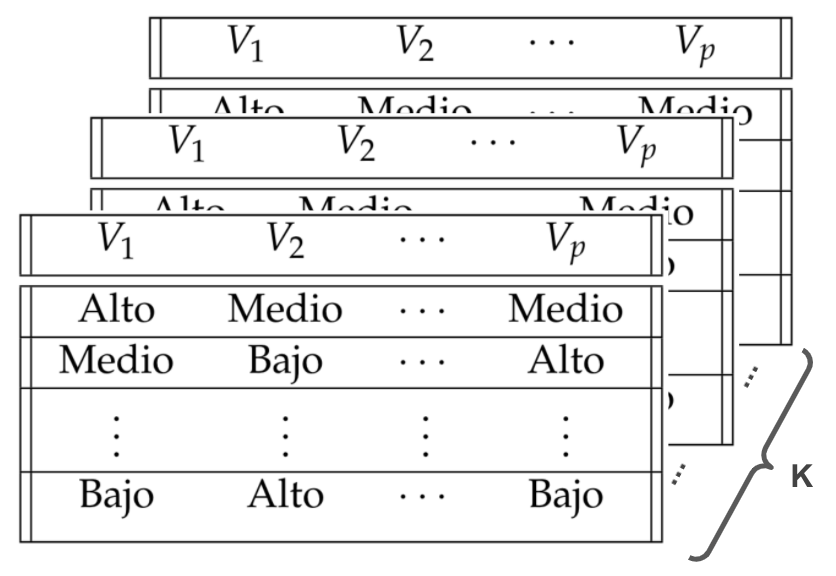
\includegraphics[width=0.4\linewidth,]{ktables} \end{center}

\caption{K tablas con el formato inicial.}

\label{fig:ktables}
\end{figure}

La generalización a K tablas del procedimiento del MCA, se presenta en
la Figura \ref{fig:MCAk}

\begin{figure}[!h]


\begin{center}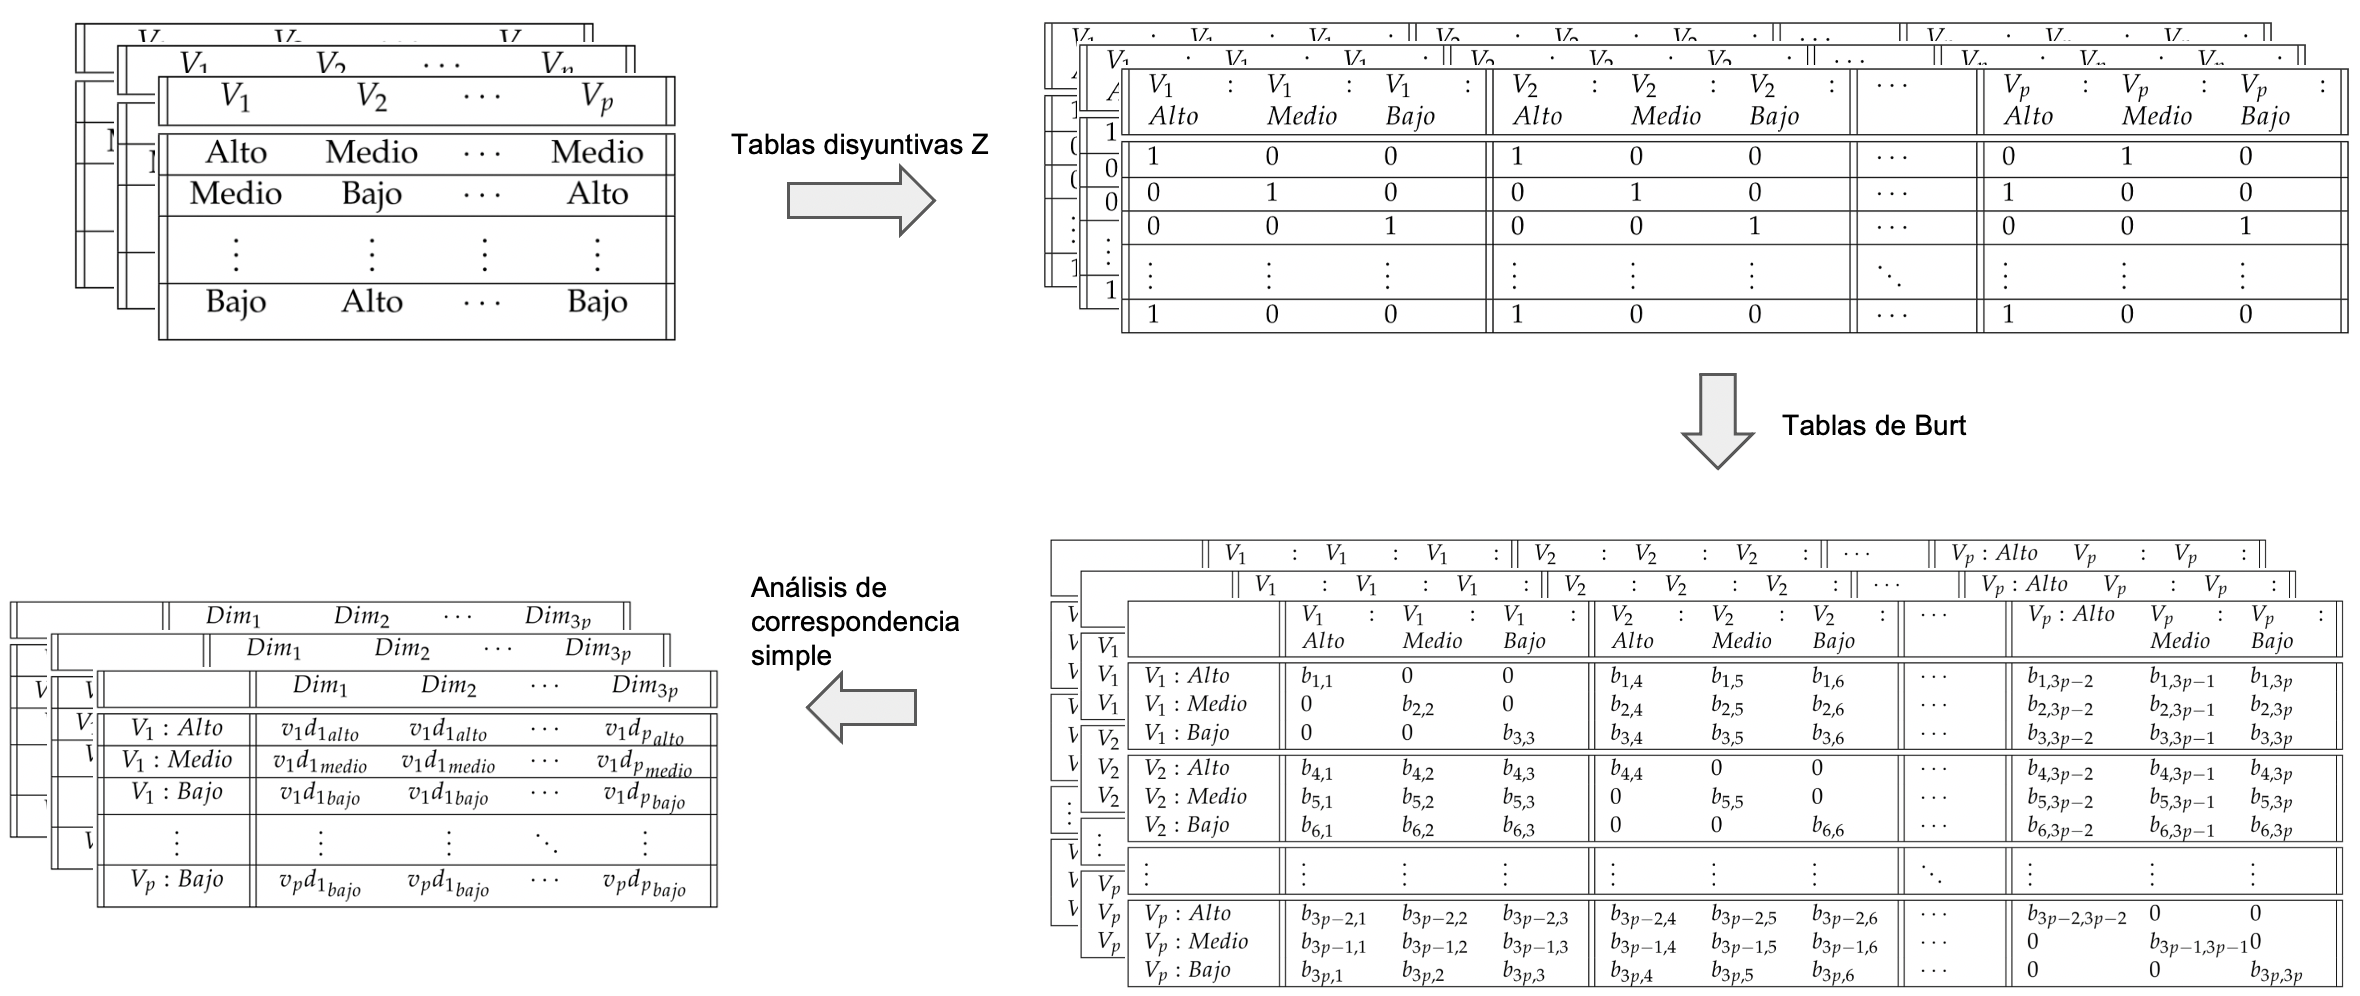
\includegraphics[width=0.9\linewidth,]{ktablesMCA} \end{center}

\caption{Procedimiento del MCA para K tablas}

\label{fig:MCAk}
\end{figure}

Se llama \(C\) a cada tabla de coordenadas. Con la finalidad de detectar
la magnitud de las variables latentes, su aporte neto a las variables,
se trata la matriz \(C\) con valor absoluto.

\hypertarget{aporte-del-anuxe1lisis-factorial-muxfaltiple-mfa}{%
\subsection{Aporte del Análisis Factorial Múltiple
(MFA)}\label{aporte-del-anuxe1lisis-factorial-muxfaltiple-mfa}}

Una vez que se tienen las coordenadas de las columnas, se procede a
realizar la normalización, característica del procedimiento MFA.

Sea \(\lambda_{1}^{k}\) el primer valor propio obtenido de la
descomposición singular de la k-ésima tabla C. Se normaliza la tabla
multiplicándola por \(1/\lambda_{1}^{k}\). Con esto se obtiene la tabla
\(C^{'}\), que corresponde a la tabla de coordenadas normalizadas.\\
Individualmente, para el caso de la matriz k, se tendría la siguiente
expresión.

\begin{equation}
\mathbf{C'_k}=\frac{1}{\lambda_{k}^1} \mathbf{C_k}
\label{eq:Cprimak}
\end{equation}

Aglomerando las matrices normalizadas \(C^{'}\) en una sola, se tiene la
matriz \(\mathbb{C}^{'}\). Esta contiene todos los elementos de las k
tablas.

\begin{equation}
\mathbf{\mathbb{C^{'}}}=[\mathbf{C_1^{'}}|\mathbf{C_2^{'}}|,...,|\mathbf{C'_{K}}]^{T}
\label{eq:Cprima}
\end{equation}

La normalización que realiza el MFA se encarga de ponderar las k tablas,
con el objetivo de evitar alguna descompensación al momento de realizar
el análisis conjunto de las tablas.

\hypertarget{gruxe1fico-de-control}{%
\subsection{Gráfico de control}\label{gruxe1fico-de-control}}

Para definir el gráfico de control \(T^2\) Hotelling se deben tomar las
siguientes consideraciones:

\begin{itemize}
\tightlist
\item
  La tabla \(\mathbb{C}^{'}\) (Ecuación \ref{eq:Cprima}) se denomina
  Consenso, sirve como referente para el escenario \emph{bajo control},
  y de la cual se obtiene \(\mu_{0}\) y \(\mathbf{S_0}\).\\
\item
  Cada matriz \(\mathbf{C'_k}\) tiene el mismo número de filas (n) y
  columnas (p) (individuos y variables).
\item
  El vector de medias \(\mathbf{\mu_k}\) está atado a la tabla
  \(\mathbf{C'_k}\), es decir, el gráfico de control estará en función
  de las diferencias entre las matrices \(\mathbf{C'_k}\) y la matriz
  consenso \(\mathbf{\mathbb{C^{'}}}\).
\item
  Las matrices \(\mathbf{C'_k}\) siguen una distribución normal
  multivariante con vector de medias \(\mu_{k}\) y matriz de covarianzas
  \(\mathbf{S_k}\).
\end{itemize}

Con esto se obtiene el estadístico \(T^2\):

\begin{equation}
T^2=n (\mu_{k}-\mu_{0})'\mathbf{\Sigma_{0}^{-1}}(\mu_{k}-\mu_{0})
\label{eq:T2}
\end{equation}

Se sabe que, bajo control, el \(T^2\) se distribuye como una
Chi-cuadrado con \(p\) grados de libertad \(\chi^2_p\). En este caso se
puede aplicar este principio, ya que se utiliza la matriz consenso
(\(\mathbb{C}^{'}\)), que representa al escenario bajo control.

Dado que este gráfico de control está basado en distancias de
Mahalanobis ponderadas, sólo tiene límite de control superior. Este
viene dado por la ecuación \ref{eq:UCL}

\begin{equation}
UCL=\chi^2_{\alpha,p}
\label{eq:UCL}
\end{equation}

donde \(p\) es el número de dimensiones y \(\alpha\) es la significancia
predeterminada considerando \(p\).

\hypertarget{tabla-posterior}{%
\subsection{Tabla posterior}\label{tabla-posterior}}

Con la finalidad de detectar las potenciales categorías responsables de
que un punto en el gráfico \(T^2\) de Hotelling para variables
cualitativas se encuentre fuera de control, se propone una tabla que
presenta las anomalías de cada categoría en cada variable, comparando
las masas de columna de la tabla \(k\) y las masas de columna de la
tabla consenso por medio de distancias \(\chi^2\) que proporcionan un
valor p, aportando a la interpretación.

\hypertarget{complemento-computacional}{%
\section{Complemento computacional}\label{complemento-computacional}}

Para facilitar la difusión y aplicación del método propuesto, se ha
desarrollado un paquete reproducible en R. El paquete \textbf{T2Qv}
utiliza la metodología expuesta en este artículo y la lleva a un entorno
práctico, permite visualizar los resultados de forma plana o
interactiva, además, presenta un panel Shiny que contiene todas las
funciones individuales en un mismo espacio.

\hypertarget{disponibilidad}{%
\subsection{Disponibilidad}\label{disponibilidad}}

El paquete está disponible en GitHub, la descarga se la puede realizar
de la siguiente forma:

\begin{verbatim}
install.packages("devtools")
devtools::install_github("JavierRojasC/T2Qv")
\end{verbatim}

\hypertarget{el-paquete-t2qv}{%
\subsection{El paquete: T2Qv}\label{el-paquete-t2qv}}

\begin{figure}[!ht]



\begin{center}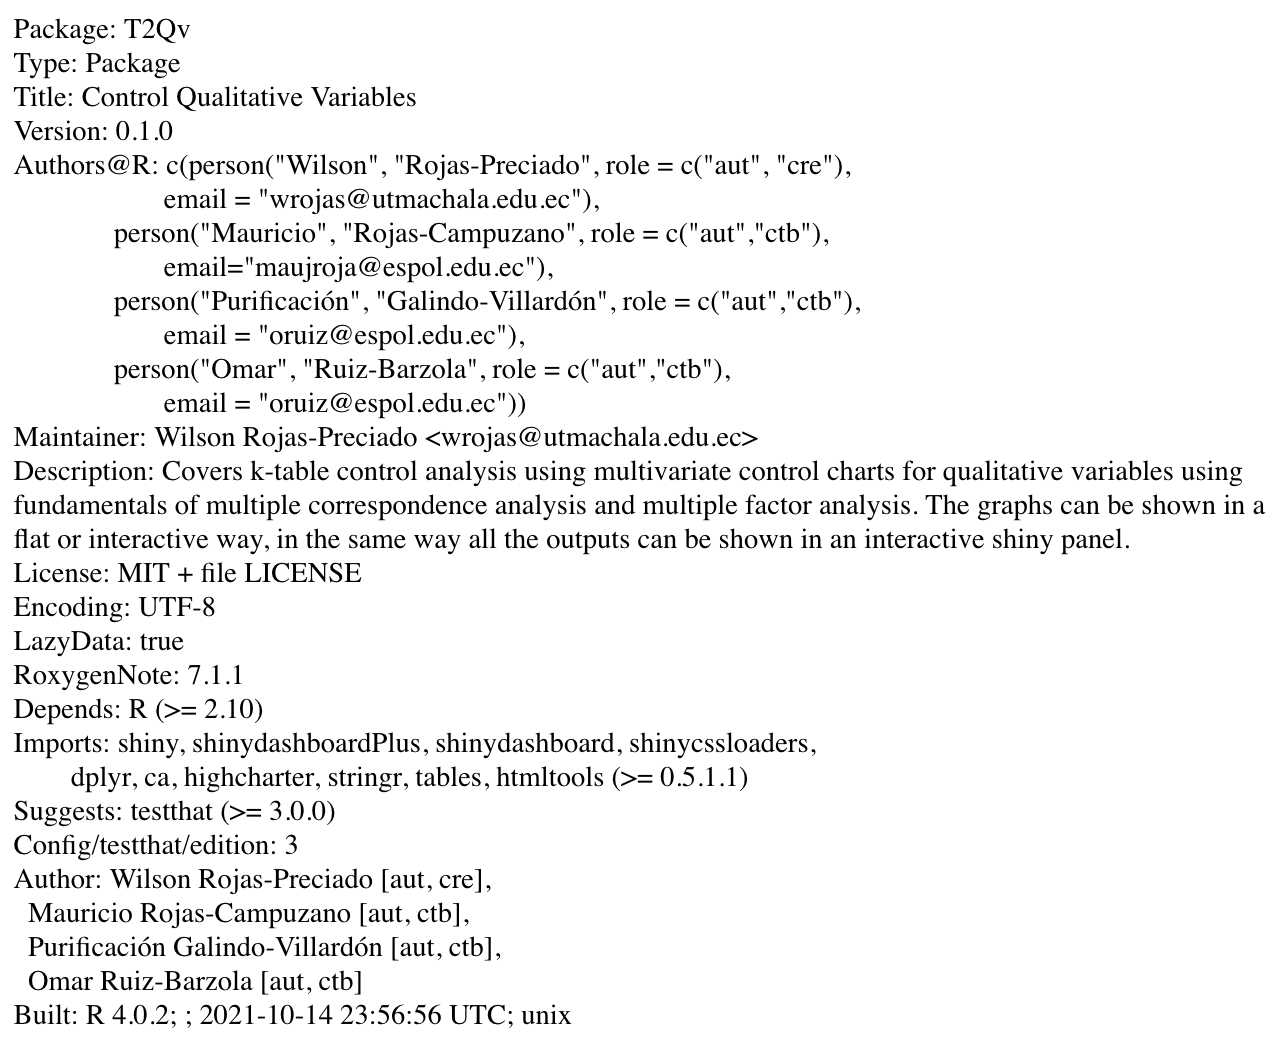
\includegraphics[width=0.6\linewidth,]{DescrPack} \end{center}

\caption{Documentación del paquete T2Qv}

\label{fig:documentation}
\end{figure}

Las funciones que contiene el paquete y su descripción se enuncian en la
tabla \ref{tab:functions}.

\begin{table}[!ht]
\begin{center}
 \begin{tabular}{||c  m{35em}||} 
 \hline
  Función & Descripción \\ [0.5ex] 
 \hline\hline
 T2 qualitative & Multivariate control chart T2 Hotelling applicable for qualitative variables.\\
 \hline
  MCAconsensus & Multiple correspondence analysis applied to a consensus table.\\
\hline
  MCApoint & Multiple correspondence analysis applied to a specific table.\\
\hline
  ChiSq variable & Contains Chi square distance between the column masses of the table specified in PointTable and the consensus table. It allows to identify which mode is responsible for the anomaly in the table in which it is located. \\ [1ex] 
  \hline
  Full Panel & A shiny panel complete with the 
  multivariate control chart for 
  qualitative variables, the two MCA 
  charts and the modality distance table. 
  Within the dashboard, arguments such as 
  type I error and dimensionality can be 
  modified. \\ [1ex] 
 \hline
\end{tabular}\caption{Funciones del paquete T2Qv}
\label{tab:functions}
\end{center}
\end{table}

\hypertarget{resultados}{%
\section{Resultados}\label{resultados}}

Con la intención de probar la metodología propuesta en el gráfico de
control \(T^2\) de Hotelling para variables cualitativas, se hizo un
análisis con datos simulados y otro con datos reales aplicados al
contexto de la educación superior. Los resultados se obtienen de la
aplicación del paquete T2Qv.

\hypertarget{resultados-con-datos-simulados}{%
\subsection{Resultados con datos
simulados}\label{resultados-con-datos-simulados}}

Para este estudio se generó una base de datos simulados, a la que se
denominó \emph{Datak10Contaminated}. Consta de 10 tablas, cada una de
ellas está constituida por 100 filas (observaciones) y 11 columnas, de
las cuales, las 10 primeras corresponden a las variables analizadas (V1,
V2, \ldots; V10) mientras que, la columna 11, denominada
\emph{GroupLetter}, contiene el factor de clasificación de los grupos.
Para su identificación, las tablas han sido denominadas con las letras
del alfabeto, desde la \emph{a} hasta la \emph{j}. La tabla \emph{j}
tiene una distribución distinta de la que tienen las otras nueve. Los
datos se expresan en tres niveles: alto, medio y bajo. La tabla \ref{}
presenta las 10 primeras filas de la base de datos
\emph{Datak10Contaminated}.

\begin{figure}[!ht]



\begin{center}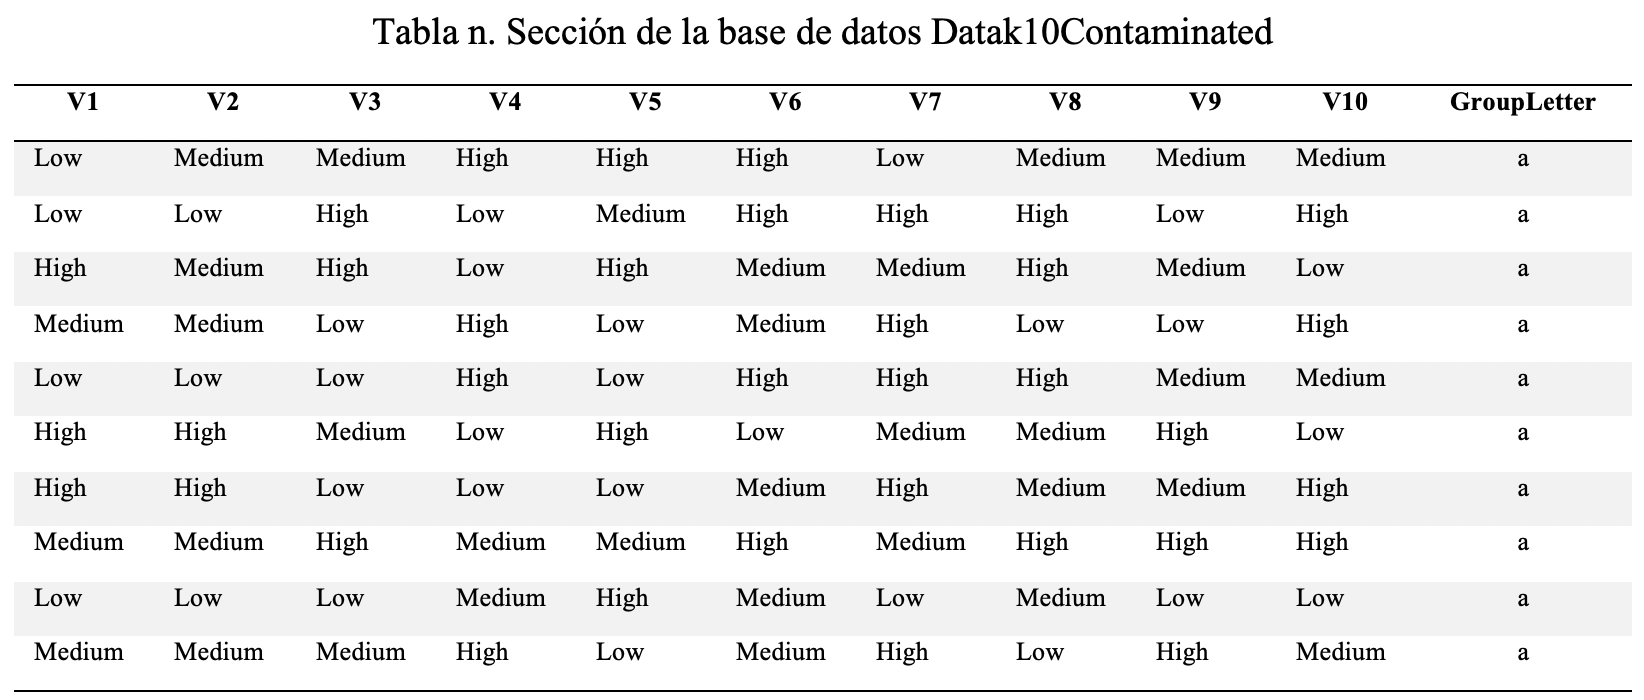
\includegraphics[width=0.6\linewidth,]{tablabase} \end{center}

\caption{Sección de la base de datos Datak10Contaminated.}

\label{tab:tabladatos}
\end{figure}

Para facilitar análisis se creó un paquete al que se denominó
\emph{T2Qv}, herramienta diseñada en el software estadístico R y R
Studio. T2Qv realiza el análisis de control de k tablas utilizando
gráficos de control multivariantes para variables cualitativas,
utilizando los fundamentos del análisis de correspondencia múltiple y el
análisis de factores múltiples. Los gráficos se pueden mostrar de forma
plana o interactiva, de la misma manera todas las salidas se pueden
mostrar en un panel interactivo de Shiny. El primer resultado es el
gráfico del Análisis de Correspondencias Múltiple (MCA) aplicado a la
tabla consenso (Figura \ref{fig:CONS1}). Esta tabla ha sido tomada como
referente, como escenario en control para el análisis posterior de las
tablas que sean reportadas como puntos fuera de control en el gráfico T2
de Hotelling. El MCA reporta una inercia total del 63.3\%, la dimensión
1 representa al 53.6\% de la información, mientras que la dimensión 2,
al 9.7\%. Los puntos del gráfico representan a las observaciones de cada
una de las 10 variables en sus tres niveles: alto, medio y bajo. En esta
figura, todas las observaciones que corresponden al nivel alto se ubican
a la izquierda en el eje de las X; de las 10 observaciones
correspondientes al nivel medio, 8 se situaron en el cuarto cuadrante y
las dos restantes en el cuadrante 1, es decir, todas las observaciones
de este nivel estuvieron a la derecha en el eje de las X. Finalmente, de
los 10 puntos que representan al nivel bajo, 8 están ubicados en el
cuadrante 1.

\begin{figure}[!ht]



\begin{center}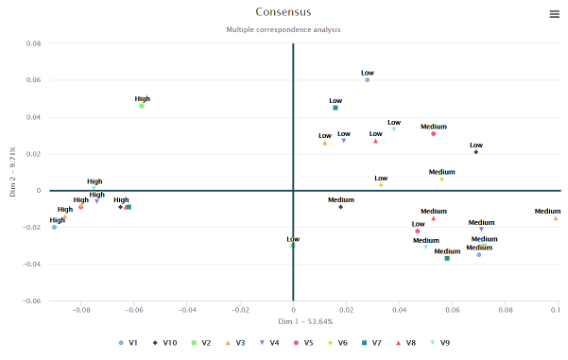
\includegraphics[width=0.6\linewidth,]{CONS1} \end{center}

\caption{Análisis de correspondencias múltiple aplicado a la tabla consenso.}

\label{fig:CONS1}
\end{figure}

Otro resultado es el Análisis de Correspondencias Múltiple aplicado a
una tabla específica. En este punto, uno de los argumentos que se debe
tener en cuenta es la selección de la tabla de la que se realizará el
análisis.

\begin{figure}[!ht]



\begin{center}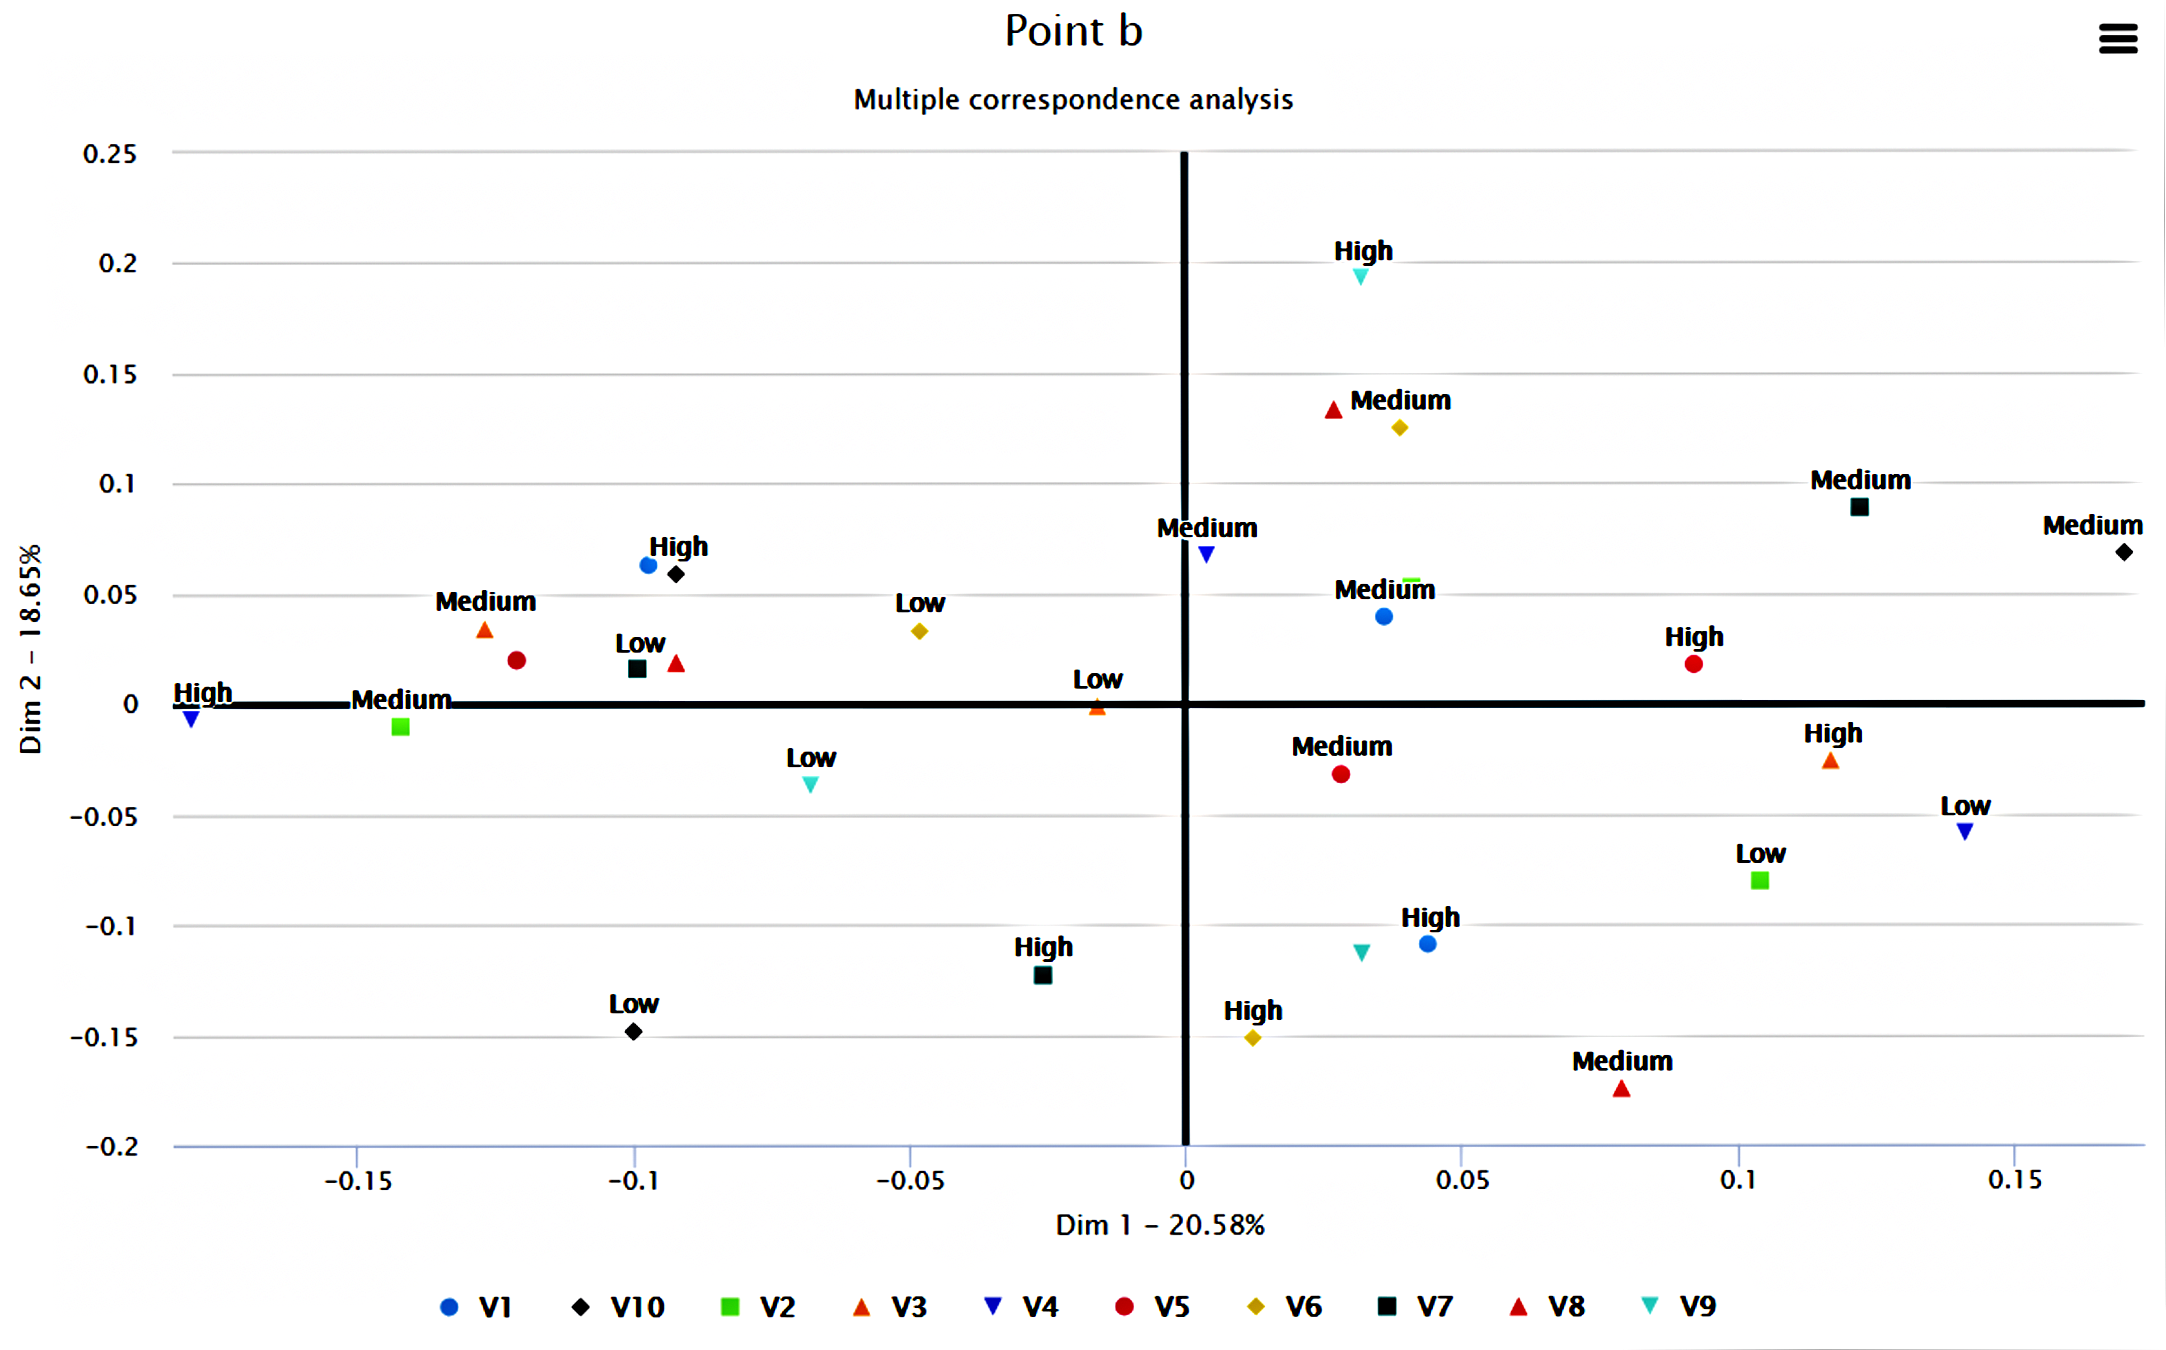
\includegraphics[width=0.6\linewidth,]{MCAb} \end{center}

\caption{Análisis de correspondencias múltiple aplicado a la tabla b.}

\label{fig:MCAb}
\end{figure}

La figura \ref{fig:MCAb} representa el gráfico del MCA de la tabla
\emph{b}. Este gráfico, en sus dos dimensiones, representa al 39.3\% de
la información. Es notorio que las observaciones en sus niveles alto,
medio y bajo están distribuidas de forma aleatoria en todos los
cuadrantes del del gráfico, no se puede precisar un patrón específico de
agrupación. Esto mismo se puede decir de los puntos representados en
cualquiera de las otras tablas, exceptuando la tabla \emph{j}, que fue
diseñada con una distribución diferente.\\
No obstante, el uso del MCA de las figuras \ref{fig:MCAb} y
\ref{fig:CONS1} todavía no permite detectar si el proceso está o no en
control. La identificación de puntos fuera de control se puede realizar
mediante la representación gráfica del estadístico T2 de Hotelling, como
se observa en la figura \ref{fig:hot1}.

\begin{figure}[!ht]



\begin{center}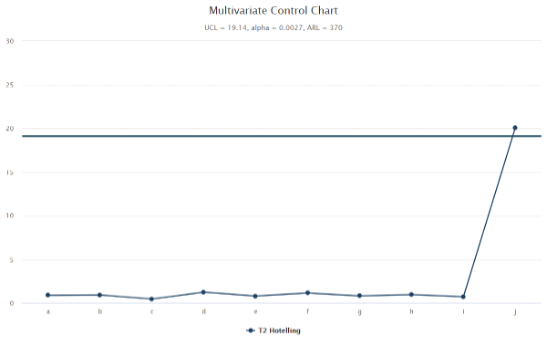
\includegraphics[width=0.6\linewidth,]{Hot1} \end{center}

\caption{Gráfico de control multivariante T2 Hotelling aplicable a variables cualitativas.}

\label{fig:hot1}
\end{figure}

La figura \ref{fig:hot1} presenta un gráfico de control elaborado con el
estadístico T2 de Hotelling, aplicado a la detección de anomalías en
cualquiera de las k tablas analizadas. Cada una de las tablas está
representada por los puntos en el gráfico. Se observa una línea
horizontal que representa al límite de control superior (UCL). El límite
de control inferior (LCL) es igual a cero.\\
Dado que el análisis de sensibilidad determinó que este gráfico de
control tiene un mejor rendimiento cuando trabaja con un número alto de
dimensiones, se ha recomendado que este sea p-1, donde p es el número de
dimensiones inicial, que es equivalente a la cantidad de variables de la
base de datos, sin contar a la variable GroupLetter que sólo sirve como
factor de clasificación de las tablas.\\
Se observa que el punto que representa a la tabla \emph{j} se ubica por
encima del límite de control superior, lo que quiere decir que se lo ha
identificado como un valor fuera de control. Por consiguiente, es
necesario analizar con detenimiento qué está pasando con los datos de la
tabla reportada, comparándolos con los de la tabla consenso, a fin de
identificar las causas de la variación y tomar las acciones pertinentes.
Para hacer un análisis del punto fuera de control se realiza un gráfico
del MCA de la tabla \emph{j} y se lo compara con el gráfico similar de
la tabla consenso, como se presenta en la figura \ref{fig:conspoint}.

\begin{figure}[!ht]



\begin{center}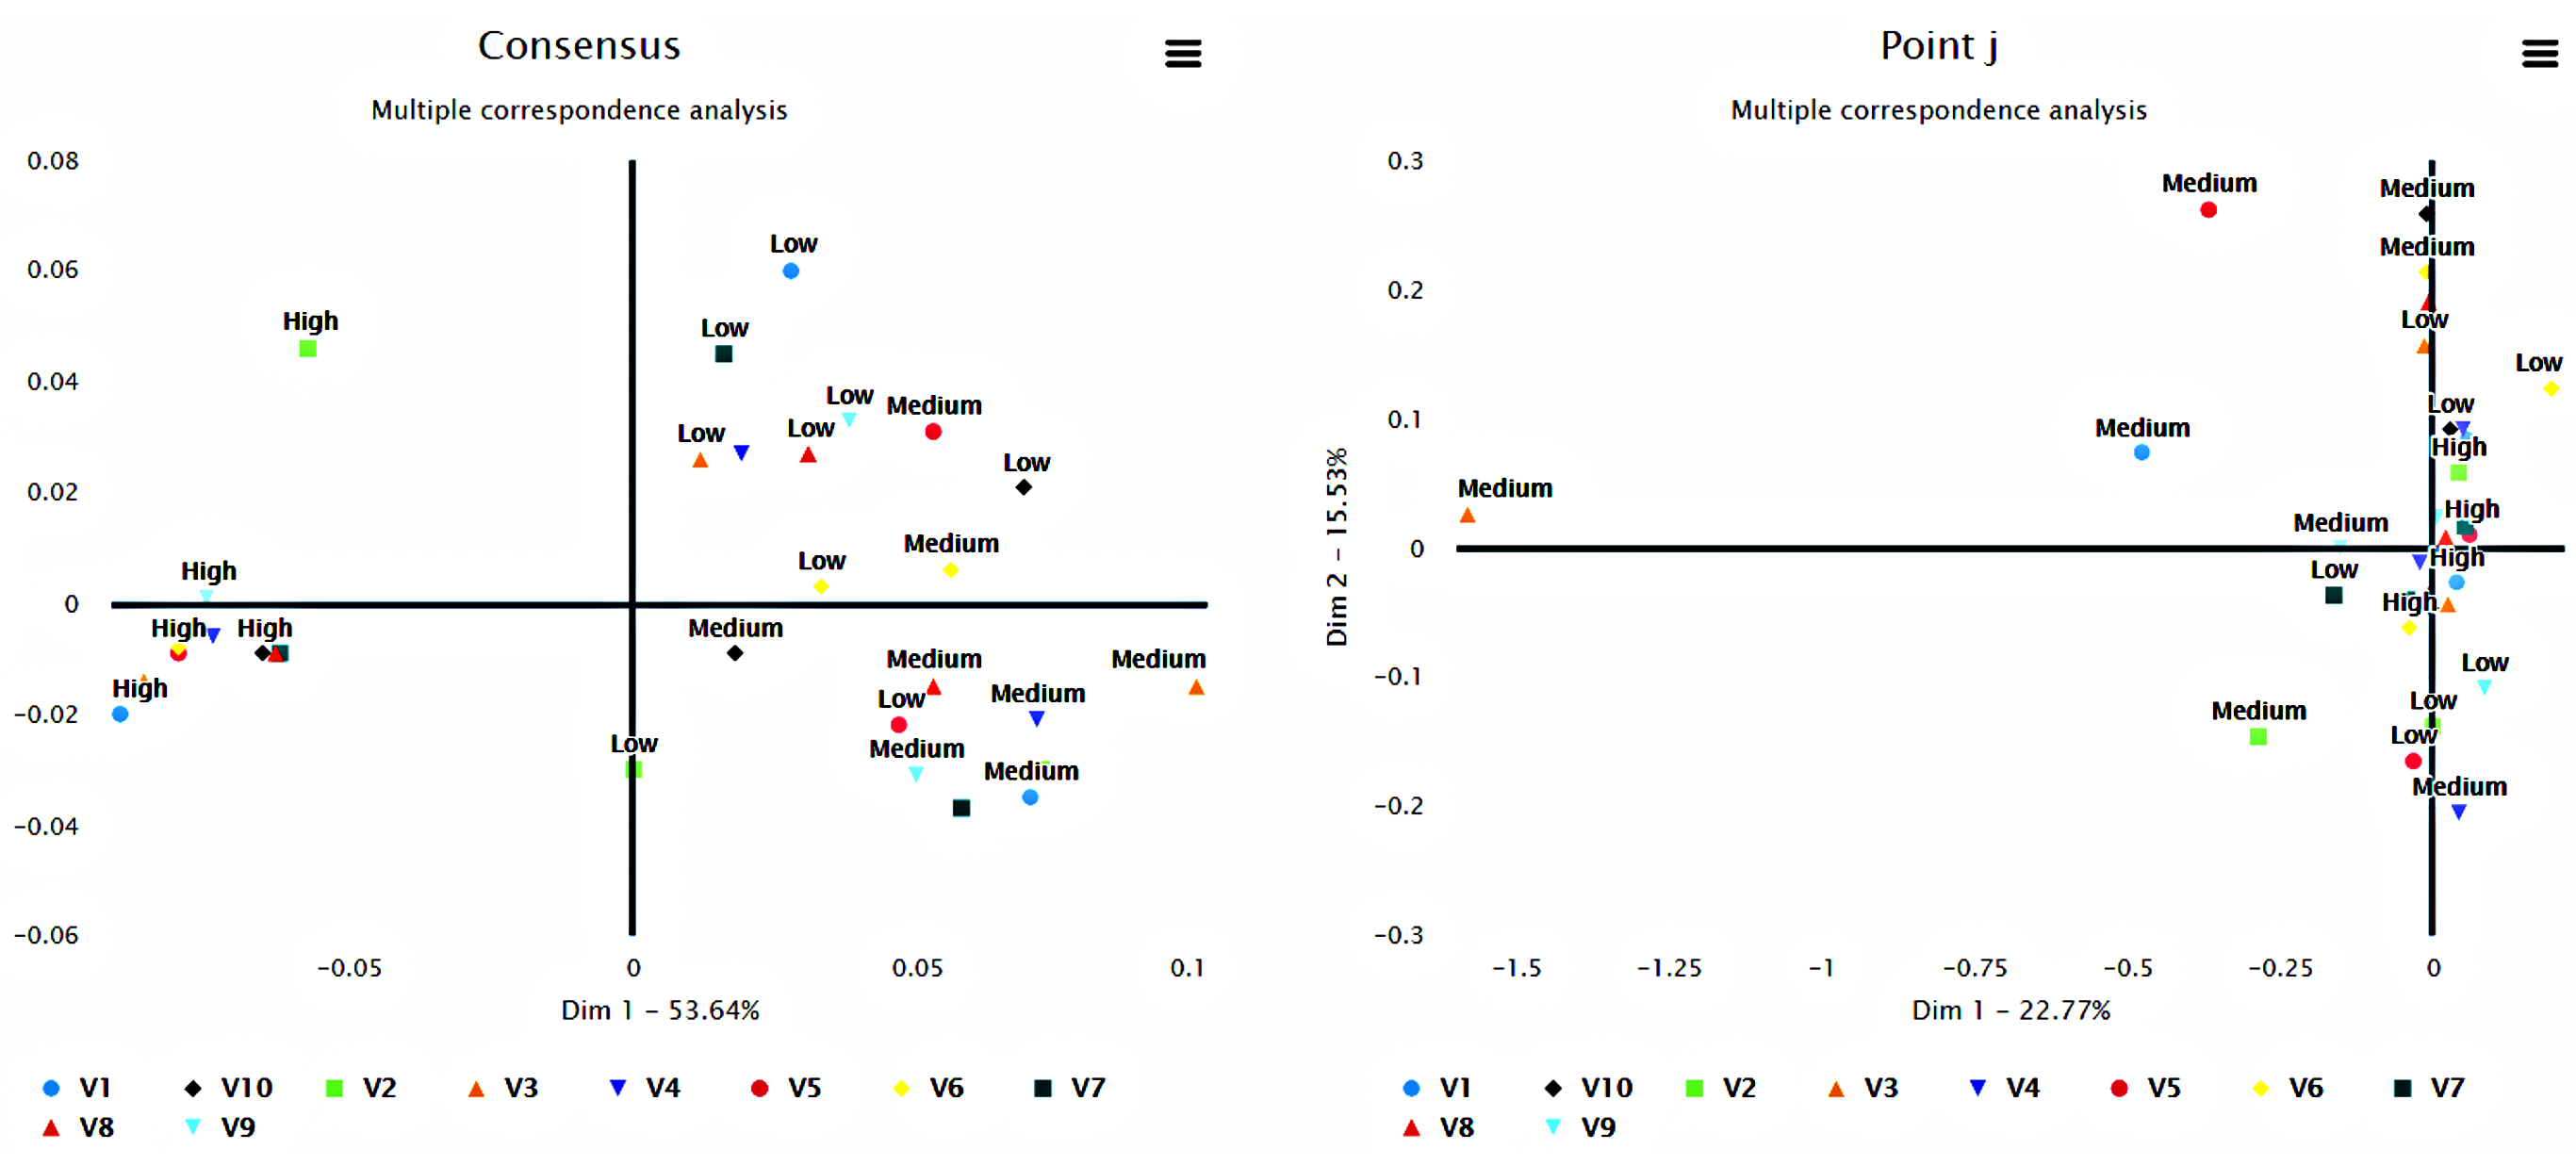
\includegraphics[width=0.6\linewidth,]{conspoint} \end{center}

\caption{Comparación de los gráficos del MCA aplicado a la tabla consenso y la tabla j.}

\label{fig:conspoint}
\end{figure}

La figura \ref{fig:conspoint} presenta la distribución de las
observaciones de las tablas consenso y \emph{j} mediante gráficos del
MCA. El gráfico de la tabla consenso, que sirve de referente en control,
ya se analizó en la figura \ref{fig:CONS1}; el de la tabla \emph{j}
muestra una tendencia de los puntos que con valores medios a ubicarse al
lado izquierdo, bastante alejados de los demás que confluyen hacia el
centro del eje de las X. Especial atención merece la variable 3, que
registra una observación para el nivel medio con el valor más alejado
del grupo.\\
Al comparar los gráficos es obvio que la distribución de los datos en la
tabla \emph{j} es diferente de las distribuciones de las demás tablas, y
en especial, es diferente de la distribución de la tabla consenso, lo
que explica por qué el punto \emph{j} ha sido identificado como fuera de
control.\\
Para profundizar en el análisis se calcula las distancias Chi-cuadrado
entre las masas de las columnas de la tabla reportada como fuera de
control y la tabla consenso, tomada como referente. Estas distancias
permiten identificar el comportamiento de las variables que inciden en
el desplazamiento de la media del proceso que finalmente pueden llevarlo
a un estado fuera de control (tabla \ref{tab:chi}).\\
La tabla \ref{tab:chi} contiene los datos de cada una de las variables
de la tabla \emph{j} con sus tres niveles (alto, medio y bajo). La
columna 3 muestra el p-valor para cada observación, de esto depende el
número de asteriscos de la columna 4 que indica el nivel de
significancia estadística. Así, si el p-valor es inferior a 0.05, la
observación se reporta como significancia estadística y va asociada a un
asterisco; si el p-valor es menor que 0.01, se entiende que hay alta
significación estadística y se registran dos asteriscos; si el p-valor
es menor que 0.001, la significancia estadística es muy alta y se
reportan tres asteriscos; caso contrario, no se reporta significancia y
la observación no lleva asteriscos.

\begin{figure}[!ht]



\begin{center}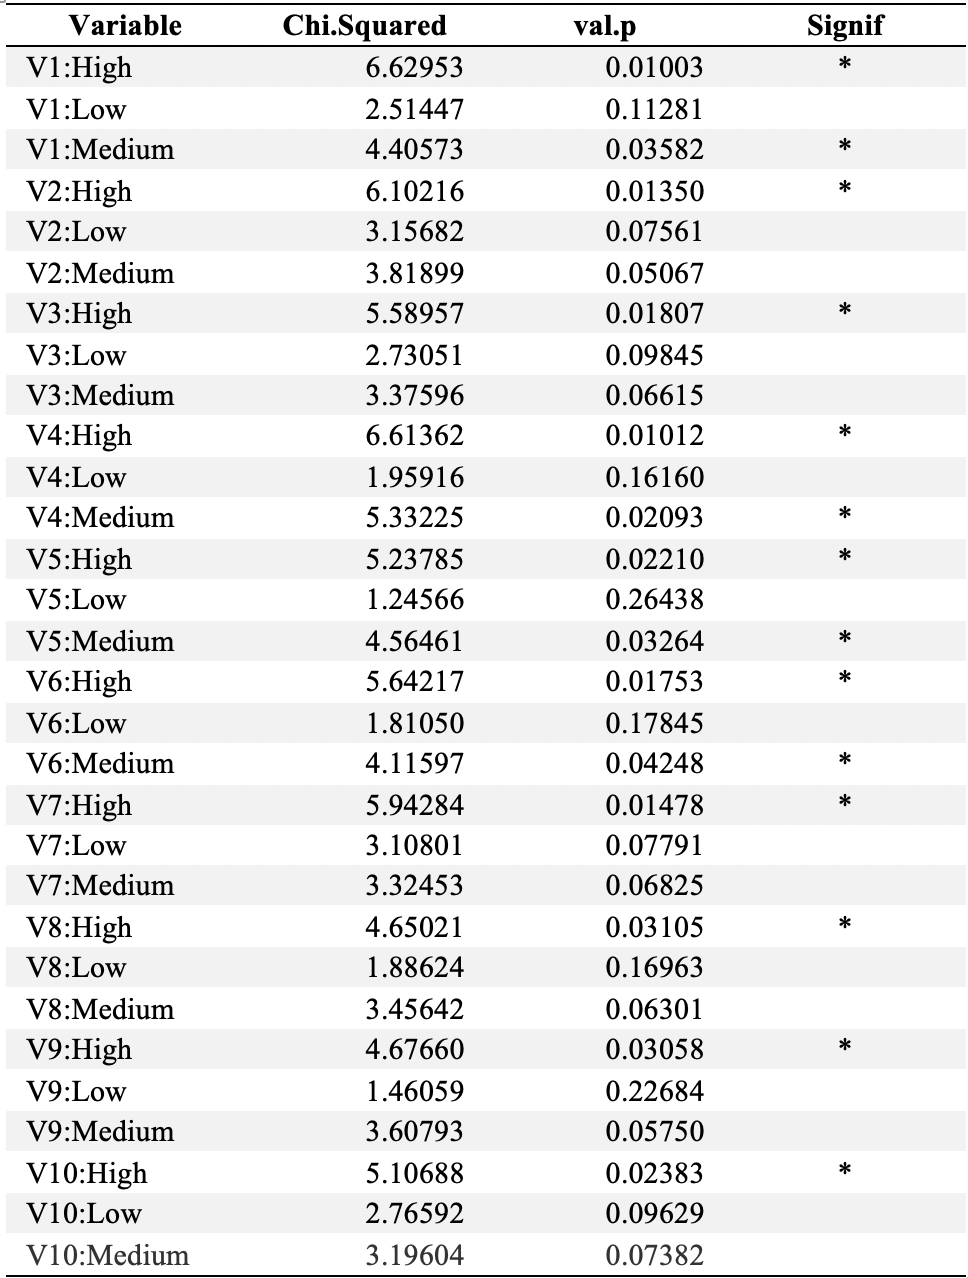
\includegraphics[width=0.6\linewidth,]{chitable} \end{center}

\caption{Distancia $\chi^2$ entre las masas de la tabla consenso y las k tablas, Datak10Contaminated}

\label{tab:chi}
\end{figure}

De las 30 observaciones que tiene la tabla \emph{j}, se presentan 14
casos de p-valores menores que 0.05, es decir, reportan significancia
estadística (un asterisco), de los cuales, 10 se atribuyen a las
categorías altas de las variables cualitativas y cuatro a los niveles
medios. El comportamiento de estas variables en la tabla \emph{j}, que
obedece a una distribución diferente a la de las demás tablas, provoca
el desplazamiento de la media del proceso que, al final, lo lleva a un
estado fuera de control. Otra manera de visualizar esta información es a
través de un gráfico de barras (figura \ref{fig:chibar}).

\begin{figure}[!ht]



\begin{center}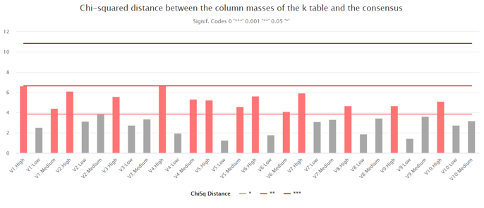
\includegraphics[width=0.6\linewidth,]{chibar} \end{center}

\caption{. Distancia $\chi^2$ entre las masas de la tabla consenso y las k tablas, Datak10Contaminated.}

\label{fig:chibar}
\end{figure}

En el gráfico de barras de la figura \ref{fig:chibar}, se observa tres
líneas horizontales que corresponden a los límites asociados a los
niveles de significancia estadística, la más baja representa al p-valor
inferior a 0.05 (un asterisco), la línea del medio, al p-valor inferior
a 0.01 (dos asteriscos); y, la línea más alta representa al p-valor
inferior a 0.001 (tres asteriscos). Las barras que representan valores
sin significancia estadística no sobrepasan ninguna de las líneas y se
pintan de color gris, mientras que, las que sí denotan significancia
estadística adquieren el color de la línea más alta que sobrepasan.

\hypertarget{resultados-con-datos-aplicados-al-contexto-de-la-educaciuxf3n-superior}{%
\subsection{Resultados con datos aplicados al contexto de la educación
superior}\label{resultados-con-datos-aplicados-al-contexto-de-la-educaciuxf3n-superior}}

En este ejemplo se utiliza una base de datos denominada
\emph{Estudiantes 2019\_2020}, tomada de reportes que la Universidad
Técnica de Machala (UTMACH) cargó en la plataforma del Sistema Integral
de Información de la Educación Superior (SIIES), correspondiente a
cuatro periodos académicos consecutivos. La base de datos
Estudiantes\_2019\_2020 contiene 43191 observaciones y 17 variables
cualitativas referidas los estudiantes de las 30 carreras vigentes en
sus 5 facultades.\\
Las variables registradas en la base de datos, con sus respectivas
categorías son las siguientes:\\
- Periodo académico, esta es la variable que sirve como clasificador,
hace referencia a 4 periodos de estudio (semestres): 2019-1, 2019-2,
2020-1 y 2020-2.

\begin{itemize}
\item
  Facultad, que tiene 5 categorías: Facultad de Ciencias Agropecuarias
  (FCA), Facultad de Ciencias Empresariales (FCE), Facultad de Ciencias
  Químicas y de la Salud (FCQS), Facultad de Ciencias Sociales (FCS) y
  Facultad de Ingeniería Civil (FIC).
\item
  Carrera, variable que contiene el nombre de las 30 carreras vigentes
  en la UTMACH, cada una de ellas es una categoría y se asocia a alguna
  de las 5 facultades. En la FCA: Acuicultura, Economía Agropecuaria,
  Agronomía y Medicina Veterinaria; en la FCE: Administración de
  Empresas, Turismo, Mercadotecnia, Contabilidad y auditoría, Comercio
  internacional y Economía; en la FCQS: Medicina, Enfermería, Bioquímica
  y Farmacia, Alimentos, Ing. Química; en la FCS: Artes plásticas,
  Pedagogía de la Actividad Física y Deporte, Pedagogía de las Ciencias
  Experimentales, Educación Básica, Educación inicial, Pedagogía de los
  Idiomas Nacionales y Extranjeros, Psicología Clínica, Psicopedagogía,
  Comunicación, Derecho, Gestión Ambiental, Sociología, Trabajo Social;
  y en la FIC: Ingeniería Civil y Tecnología de la Información.
\item
  Sexo, con sus dos clases: hombre y mujer.
\item
  Grupo edad, que clasifica a los estudiantes en 5 grupos según su edad
  en años: Menores que 18, de 18 a 30, de 31 a 45, de 46 a 60 y Mayores
  a 60.
\item
  Discapacidad, cuyas clases son: Intelectual, Auditiva, Física Motora,
  Visual, Lenguaje y Ninguna.
\item
  Etnia, con sus tipos: Mestizo, Montubio, Negro, Blanco, Indígena,
  Mulato, Afroecuatoriano, Otro, No registra.
\item
  Zona residencial, Urbana y Rural.
\item
  Nivel de formación del padre: Centro de alfabetización, Educación
  Básica incompleta, Educación Básica, Bachillerato, Superior
  tecnológica incompleta, Superior tecnológica, Superior universitaria,
  Superior universitaria incompleta, Diplomado, Especialidad, Postgrado
  Maestría o Especialización en áreas de Salud, Postgrado Ph.D., Ninguno
  y No sabe, no registra.
\item
  Nivel de formación de la madre: Centro de alfabetización, Educación
  Básica incompleta, Educación Básica, Bachillerato, Superior
  tecnológica incompleta, Superior tecnológica, Superior universitaria,
  Superior universitaria incompleta, Diplomado, Especialidad, Postgrado
  Maestría o Especialización en áreas de Salud, Postgrado Ph.D., Ninguno
  y No sabe, no registra.
\item
  Número de miembros del hogar, con sus tres clases: Hasta 3, 4 y 5 o
  más.
\item
  Tipo colegio: Fiscal, Particular, Fiscomisional, Extranjero, Municipal
  y No registra.
\item
  Ingreso total hogar: Rango 1, Rango 2, Rango 3, Rango 4, Rango 5,
  Rango 6, Rango 7, Rango 8, Rango 9 y Rango 10.
\item
  Origen de recursos estudios: Padres tutores, Hermanos y familiares,
  Pareja sentimental, Recursos propios, Beca estudio, Crédito educativo
  y No registra.
\item
  Segunda matrícula: Sí y No.
\item
  Tercera matrícula: Sí y No.
\item
  Terminó periodo: Sí y No.
\end{itemize}

\hypertarget{anuxe1lisis-de-correspondencias-muxfaltiple-de-la-tabla-consenso}{%
\subsubsection{Análisis de Correspondencias Múltiple de la tabla
Consenso}\label{anuxe1lisis-de-correspondencias-muxfaltiple-de-la-tabla-consenso}}

El gráfico del Análisis de Correspondencias Múltiple que se realiza a la
tabla consenso (Figura \ref{fig:CONS1}) es el escenario bajo control que
se utilizará para el análisis de las tablas que luego se registren como
puntos fuera de control en el gráfico T2 de Hotelling. El MCA reporta
una inercia total del 30.31\%. Los puntos del gráfico representan a las
observaciones de cada una de las 16 variables en sus distintos niveles.
La variable Periodo académico sirve como elemento clasificador, por eso
sus observaciones no aparecen aquí.

\begin{figure}[!ht]



\begin{center}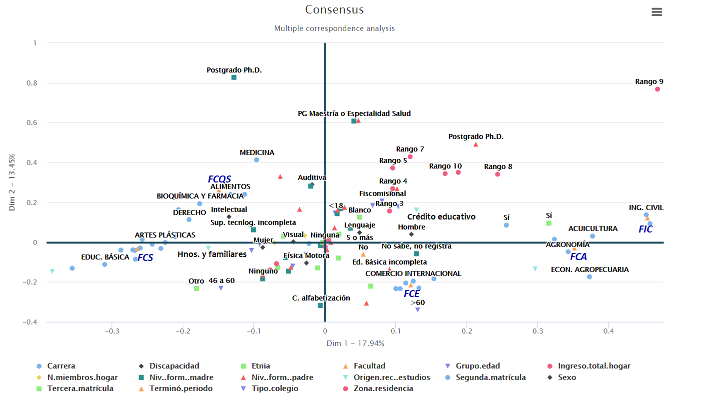
\includegraphics[width=0.6\linewidth,]{consedu} \end{center}

\caption{Gráfico de MCA de la tabla consenso, Estudiantes 2019-2020.}

\label{fig:CONSedu}
\end{figure}

Se observa cómo las carreras se agrupan alrededor de sus respectivas
facultades; la FIC y la FCA se muestran similares entre sí y ubicadas al
lado derecho, en el plano que corresponde a la dimensión 1, mientras
que, al otro extremo está la FCS. Por otra parte, las similitudes y
diferencias entre las otras dos facultades giran en torno a los ejes de
las dos dimensiones, la FCE ubicada en el cuadrante 4 y la FCQS, en el
2.\\
La variable Sexo es una de las que más incide en la ubicación de los
puntos alrededor de la dimensión 1. El número de estudiantes varones es
mayor que el de las mujeres en las carreras de la FCA y FIC, por otra
parte, el número de mujeres es mayor que el de hombres en las carreras
de la FCS y FCQS; en la FCE parece no haber marcada diferencia en la
proporción de hombres y mujeres. Las variables Segunda matrícula y
Tercera matrícula dan cuenta de que es muy frecuente que los estudiantes
aprueben sus asignaturas en su primera matrícula, sin repetir; se
observa también que la segunda y tercera matrícula ocurren con mayor
frecuencia en la FCA y la FIC, especialmente en ésta, lo que podría
estar asociado al grado de dificultad propio de las asignaturas que allí
se estudia, a procesos con mayor rigor académico y hasta a
insuficiencias en los procesos de enseñanza -- aprendizaje. Al otro
extremo está la FCS, en la que no es usual que ocurran segundas o
terceras matrículas.\\
La variable Ingreso total hogar se desplaza desde el nivel más bajo
(Rango 1), que se encuentra cercano a las carreras de la FCS, FCQS,
hasta los más altos, que corresponden a las carreras de la FCA y FIC.
Los valores medios - altos (Rangos 5, 7) están cercanos a la carrera de
Medicina en la FCQS. Las carreras del área social son preferidas por
estudiantes que provienen de familias con bajos ingresos, lo cual es
congruente con la observación de que las becas de estudio, de la
variable Origen recursos estudio, se han direccionado de manera
preferente a estudiantes de la FCS.\\
Por otra parte, se observa que la mayoría de los estudiantes de la
universidad reside en zonas urbanas, pero la categoría Zona rural se
acerca más a las carreras de la FCS. Además, los estudiantes de la FCS y
FCE provienen, mayoritariamente, de colegios fiscales y municipales; los
niveles de formación académica de padres y madres de los estudiantes son
más bajos en estos grupos, donde es usual encontrar casos de educación
básica incompleta, formación en centros de alfabetización y ninguna
formación. Los estudiantes que provienen de colegios particulares y
fiscomisionales están con mayor frecuencia en las carreras de la FCQS,
FCA y FIC; asimismo, los niveles más altos de formación de los padres y
madres, como Postgrado Ph. D, Maestrías y Especializaciones médicas se
asocian a carreras como Medicina e Ingeniería Civil. El análisis de las
variables que se manifiestan con mayor presencia en la dimensión 2 del
MCA indica que los grupos de estudiantes más jóvenes prefieren carreras
relacionadas con las ciencias médicas y de la salud, ciencias naturales
y exactas, ingenierías y tecnologías y ciencias agrícolas; mientras que,
los grupos de mayor edad se asocian a carreras que se ubican en el área
de las ciencias sociales y las humanidades. La FCA y FIC reportan menor
frecuencia de casos de estudiantes con discapacidades que las demás
facultades.

\hypertarget{gruxe1fico-de-control-multivariante-t2-hotelling}{%
\subsubsection{Gráfico de control multivariante T2
Hotelling}\label{gruxe1fico-de-control-multivariante-t2-hotelling}}

\begin{figure}[!ht]



\begin{center}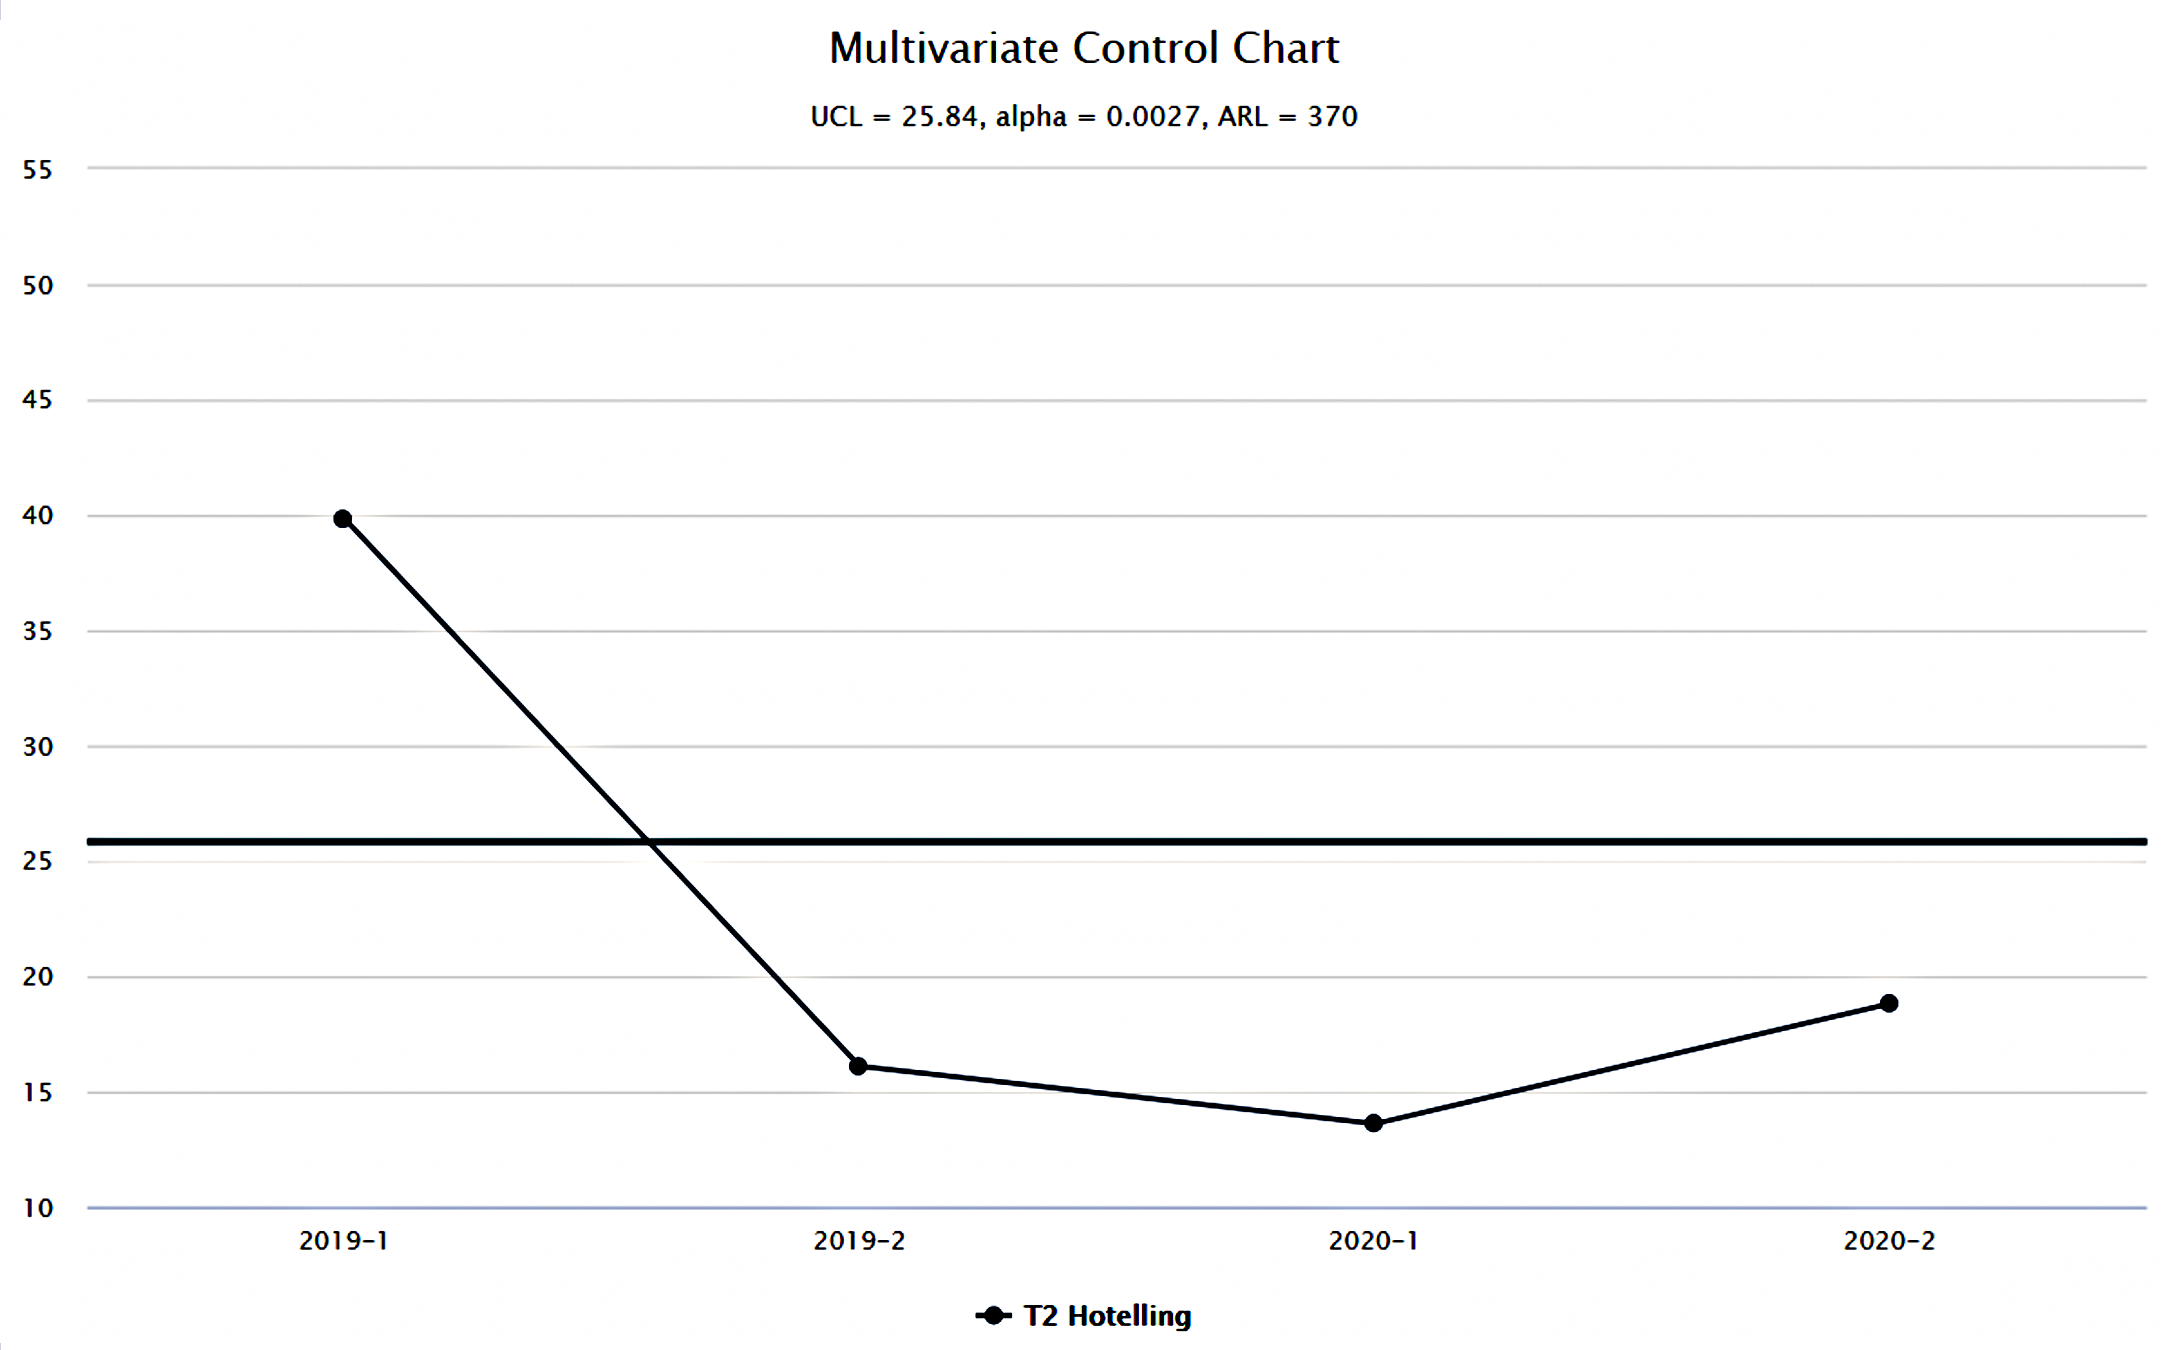
\includegraphics[width=0.6\linewidth,]{t2edu} \end{center}

\caption{Gráfico de control T2 Hotelling aplicado a las tablas de los periodos académicos analizados.}

\label{fig:t2edu}
\end{figure}

La figura \ref{fig:t2edu} muestra el gráfico de control T2 de Hotelling
para la representación de las k = 4 tablas analizadas, éstas se
representan por los puntos del gráfico y corresponden a los cuatro
periodos académicos considerados en este estudio. El punto que
representa al periodo académico 2019-1 ha sido reportado como un valor
fuera de control, en consecuencia, será necesario un análisis de sus
datos comparados con los de la tabla consenso (Figura \ref{fig:CONSedu})
para identificar las causas de la variación y, si fuera el caso, tomar
las acciones pertinentes. Para ello se realiza un MCA a la tabla 2019-1.

\begin{figure}[!ht]



\begin{center}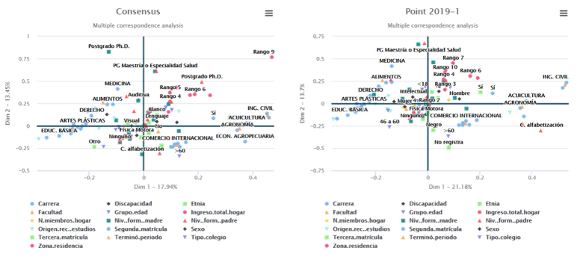
\includegraphics[width=0.6\linewidth,]{conspointedu} \end{center}

\caption{Comparación de los gráficos del MCA aplicado a la tabla consenso y la tabla 2019-2.}

\label{fig:conspointedu}
\end{figure}

La figura \ref{fig:conspointedu} contiene los gráficos del MCA de la
tabla consenso y la tabla 2019-1. Los puntos allí registrados
corresponden a las 16 variables cualitativas con sus respectivas
categorías. Se ve que hay puntos que conservan su ubicación o que han
variado muy poco en ambas tablas, como las facultades, carreras, la
variable Sexo y la Zona residencia. Además, se observa categorías de
variables que han cambiado su ubicación de manera sensible y que pueden
estar ocasionando el estado fuera de control. La identificación de estas
tablas se facilita cuando se analiza la figura \ref{fig:conspointedu}.

\begin{figure}[!ht]



\begin{center}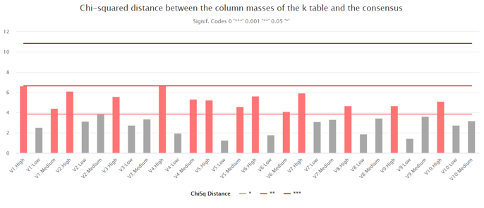
\includegraphics[width=0.6\linewidth,]{chibar} \end{center}

\caption{Distancia $\chi^2$ entre las masas de la tabla consenso y las k tablas, Estudiantes 2019 2020.}

\label{fig:conspointedu}
\end{figure}

La figura \ref{fig:conspointedu}, permite apreciar, en un gráfico de
barras, la distancia Chi cuadrado entre las categorías de la tabla
consenso y de la tabla 2019-1, reportada como fuera de control. Mientras
más altas son las barras, mayor es esta distancia. Las barras que
sobresalen representan a las variables que, en la comparación, tienen
una distribución muy distinta, de manera que han alcanzado significancia
estadística muy alta y p-valores inferiores a 0.001 (tres asteriscos),
por eso han adoptado el color correspondiente a ese nivel en el gráfico.
Estas variables son las que con mayor fuerza están provocando el
desplazamiento de la media del proceso y llevando al punto a un estado
fuera de control. En consecuencia, es en ellas que se debe profundizar
el análisis comparativo mediante el MCA.

\begin{figure}[!ht]



\begin{center}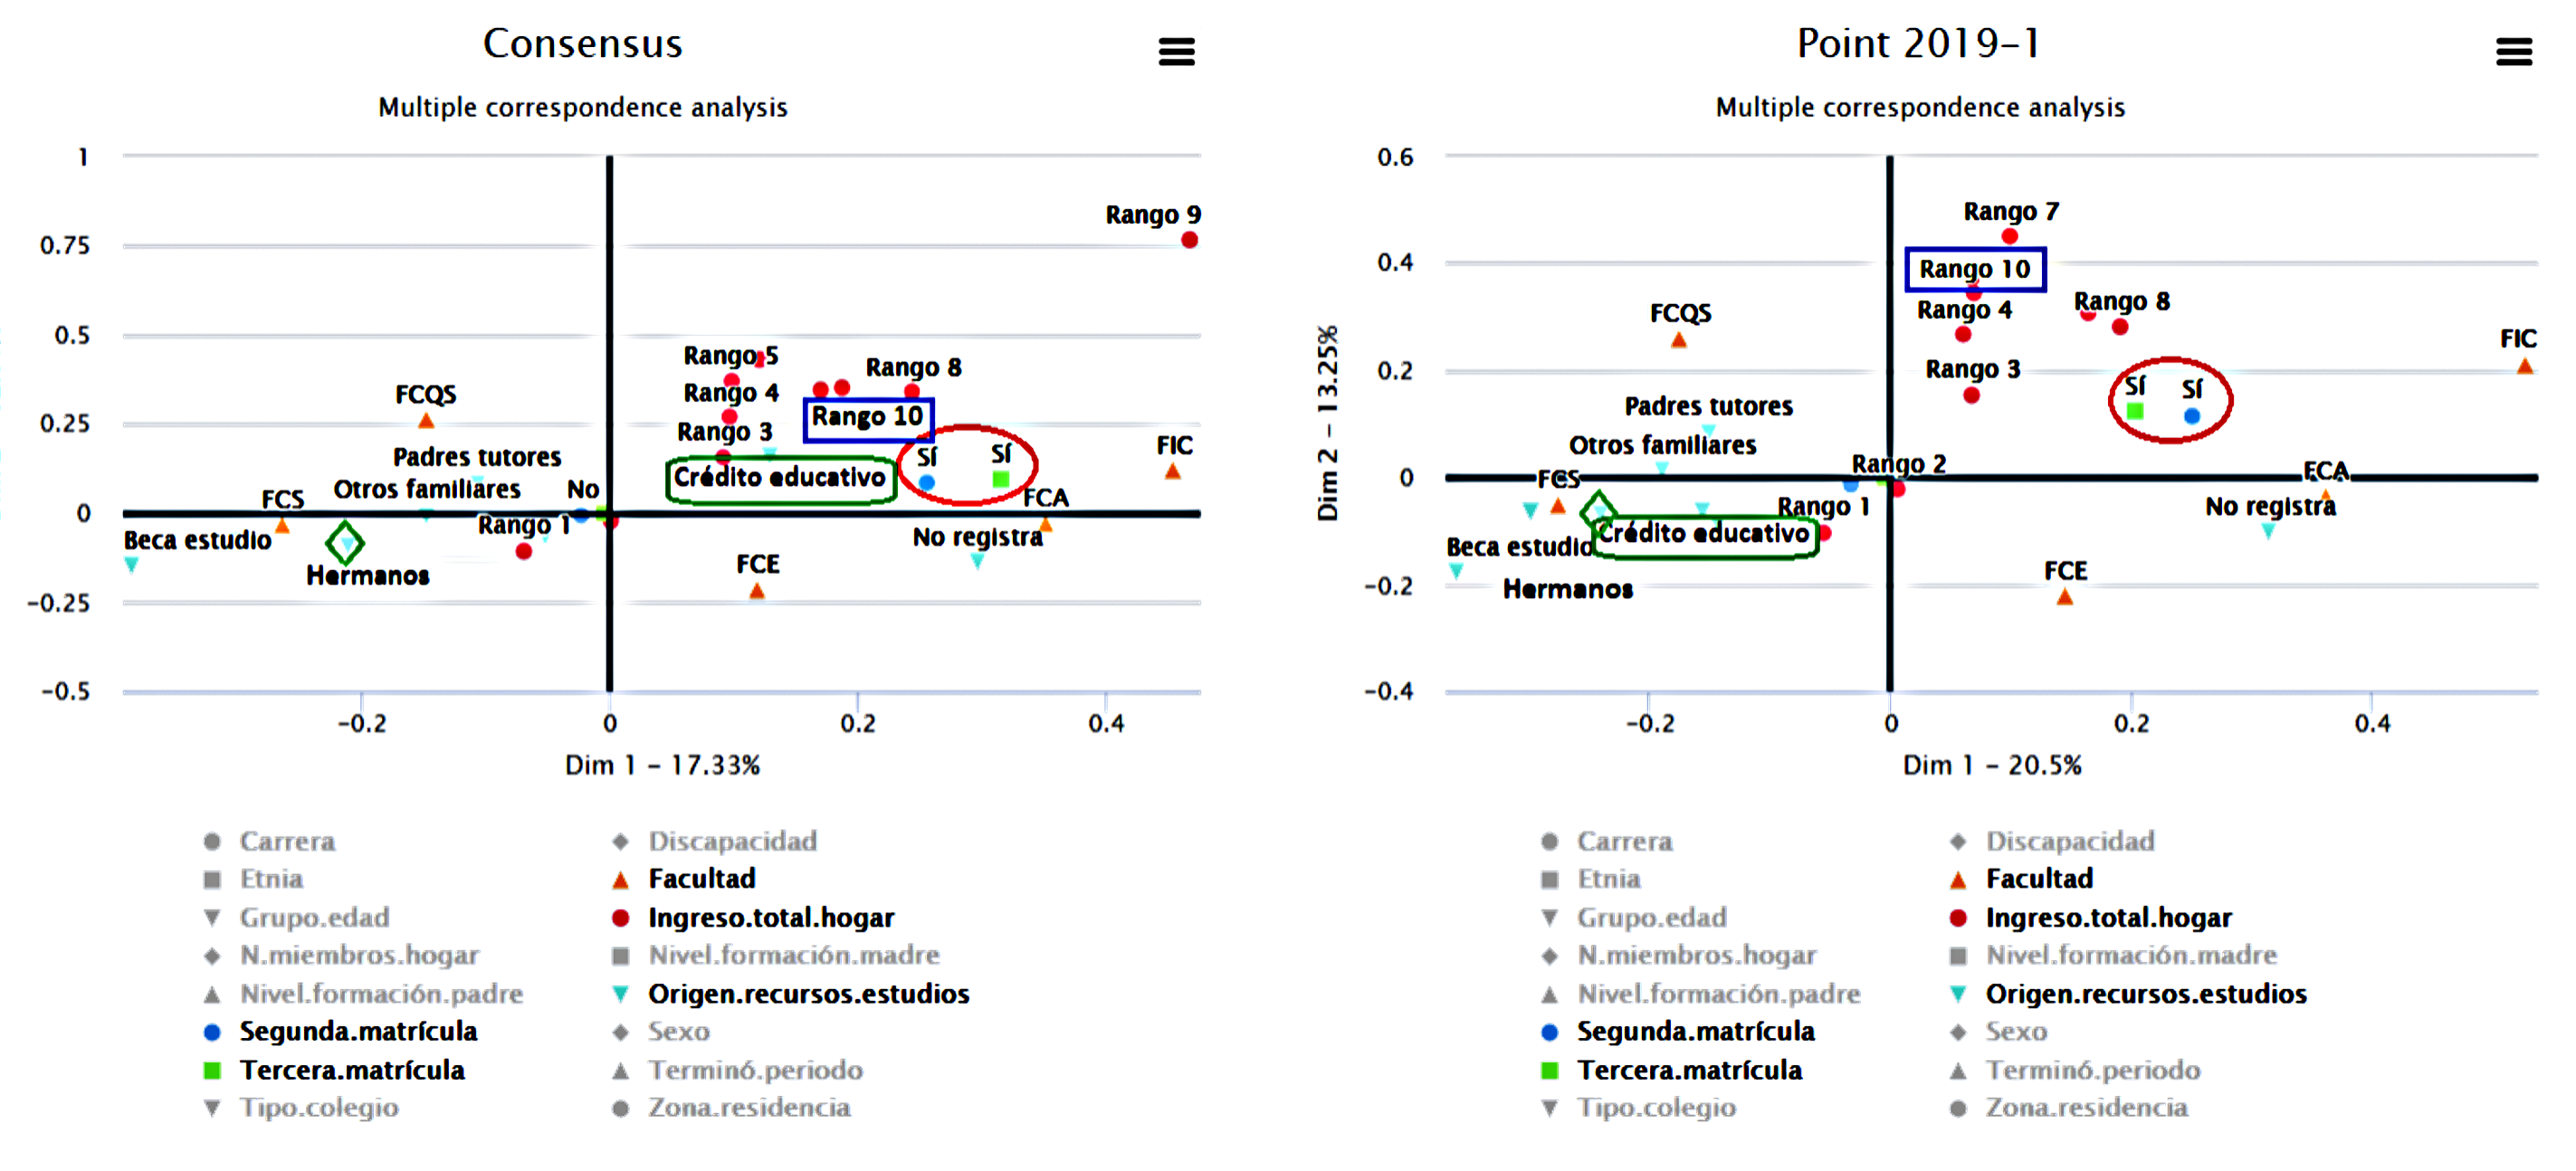
\includegraphics[width=0.6\linewidth,]{mcacompedu} \end{center}

\caption{Comparación de los gráficos del MCA con énfasis en las variables de mayor significancia estadística.}

\label{fig:mcapointedu}
\end{figure}

En la figura \ref{fig:mcapointedu}, la barra más alta representa a la
categoría Rango 9 de la variable Ingreso total hogar, que se ubica en la
esquina superior del cuadrante 1 en la tabla consenso, pero, ya no
aparece en la tabla 2019-1. Las categorías Rango 8 y Rango 10 tuvieron
un desplazamiento hacia la izquierda. Durante el periodo de estudio, los
estudiantes que provienen de familias con ingresos más altos han ido
migrando desde Ingeniería Civil, Tecnologías de la Información,
Acuicultura, Medicina Veterinaria y Agronomía, hacia carreras como
Medicina e Ingeniería Química; los de ingresos medios se van alejando de
las carreras como Administración de Empresas, Economía, Contabilidad y
Auditoría, mientras que los estudiantes de bajos recursos no han
modificado su preferencia: Carreras de Educación, Sociología y Trabajo
Social.\\
Otra variable que demuestra alta incidencia en el desplazamiento de la
media del proceso es Origen recursos estudios. Se observa que la
categoría Crédito educativo demuestra un desplazamiento considerable, en
la tabla consenso se ubica en el primer cuadrante, mientras que, en la
tabla 2021-1 aparece en el tercero (figura \ref{fig:mcapointedu}). Esto
implica que el crédito educativo que se ofrece a los estudiantes ha
cambiado de dirección, desde áreas relacionadas con las ciencias
sociales y humanísticas hasta áreas administrativas, ingenierías,
tecnologías y ciencias agrícolas. Por otra parte, la categoría Hermanos
y familiares se mantiene cerca de las carreras de la FCS, lo que
significa que los estudiantes de bajos recursos que estudian carreras de
áreas sociales y humanísticas obtienen ayuda económica de sus
familiares.\\
El nivel Postgrado Ph.D.~de las variables Nivel de formación del padre y
Nivel de formación de la madre manifiesta diferencias altamente
significativas en los dos gráficos de MCA, pues sólo aparece en la tabla
consenso, no en la 2019-1. Esto se entiende porque a principios de 2019
todavía no había padres de familia de la UTMACH que ostentaran ese grado
académico, y en la comunidad general eran pocos. No obstante, con el
transcurso del tiempo varios de ellos, que estaban en proceso de
formación de doctorado, han logrado titularse, además, otros padres de
familia que ya tenían tal grado académico han matriculado a sus hijos en
esta universidad.\\
Al hacer un análisis del comportamiento de la variable Etnia en los años
2019 - 2020, llama la atención que estudiantes que se autodefinieron
como Negros, Afroecuatorianos y Mulatos, se alejan de carreras de áreas
sociales y humanísticas para acercarse a otras del área administrativa,
como Administración de Empresas, Contabilidad y Auditoría, Comercio
internacional, Turismo, Mercadotecnia y Economía. Mientras que,
estudiantes que se autodenominaron Indígenas, migraron desde éstas hacia
otras carreras en áreas sociales y humanísticas.\\
Como cambios relevantes en torno a la variable Discapacidad se tiene
que, en los periodos académicos 2019-1 hasta 2020-2, la discapacidad
Intelectual se acerca a la carrera de Derecho; la discapacidad Auditiva,
a la Ingeniería química, Alimentos y Medicina. Mientras tanto, disminuye
la frecuencia de estudiantes con discapacidad Visual en Gestión
Ambiental, Artes plásticas y Pedagogía de la Actividad Física y Deporte.

\hypertarget{anuxe1lisis-de-sensibilidad}{%
\section{Análisis de sensibilidad}\label{anuxe1lisis-de-sensibilidad}}

Como se ha mencionado, en el gráfico T2Qv un punto fuera de control se
interpreta como una tabla (\(k_i\)) que incluye una cantidad o una
proporción de variables contaminadas, de tal manera que la diferencia de
los valores de masas de columna, entre de la matriz \(k_i\) y la matriz
consenso, sean significativos según el valor \(p\) obtenido de la
distribución \(\chi^2\). En estos casos, se espera que los puntos en el
gráfico T2Qv generalicen el comportamiento de estas diferencias y
superen el límite de control superior (\emph{UCL}). La ubicación de este
límite de control varía en función del número de dimensiones que se
representen, así, cuando es alto se logra un desempeño óptimo, mientras
que, se introduce inestabilidad y se pierde confiabilidad en los
resultados al disminuir el número de dimensiones de entre las que se
puede representar.

El gráfico de control propuesto es capaz de detectar un punto fuera de
control, aún con un bajo número de variables contaminadas, cuando se
trabaja con un alto número de dimensiones. Se recomienda \(p\) - 1, tal
que \(p\) es el número total de dimensiones de la matriz inicial (Tabla
\ref{tab:inicial}). Cuando se disminuye el número de dimensiones también
disminuye la altura del límite de control superior (\emph{UCL}), en
consecuencia, se incrementa el número de puntos fuera de control, aunque
no necesariamente las variables expresen diferencias significativas en
su valores, crece la probabilidad de falsos positivos.\\
Por consiguiente, la pregunta que surge es hasta cuántas dimensiones se
puede disminuir en el análisis sin perder confiabilidad en el resultado.
La importancia de esta pregunta radica en la necesidad de disponer un
gráfico confiable, que identifique puntos fuera de control aún si se ha
aplicado a los datos una técnica de una reducción de dimensiones, sin
caer en casos de falso positivo.

\begin{figure}[!ht]



\begin{center}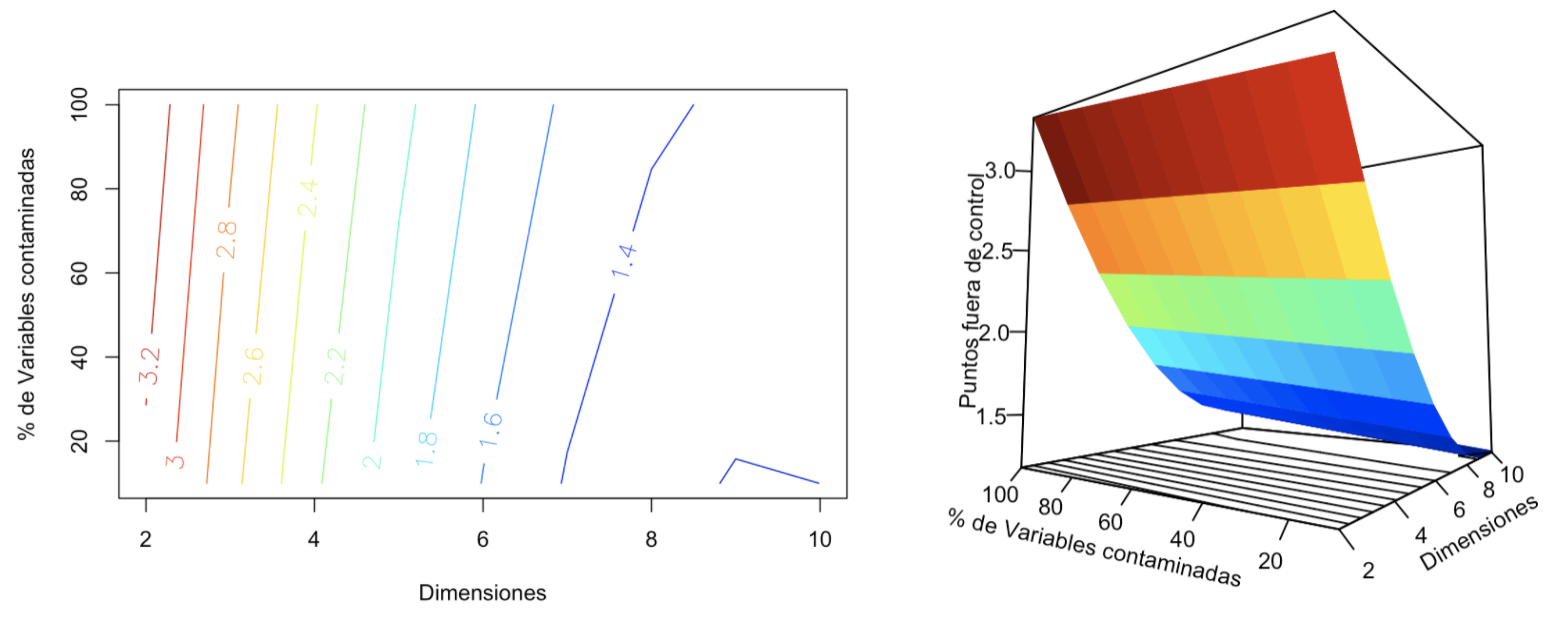
\includegraphics[width=0.8\linewidth,]{conjuntosensibilidad} \end{center}

\caption{Curvas de nivel y superficie de respuesta obtenidas con el gráfico T2 Hotelling para variables cualitativas.}

\label{fig:sensibilidad}
\end{figure}

El análisis de sensibilidad utiliza curvas de nivel y superficies de
respuesta (figura \ref{fig:sensibilidad}) para representar el número de
puntos fuera de control, considerando el porcentaje de variables
contaminadas de la \(k_i\) tabla y el número de dimensiones
representadas. Los datos de prueba utilizados en el modelo se registran
en 10 tablas, cada una de ellas incluye 10 variables y cada variable
tiene tres categorías: alto, medio y bajo. La tabla 10 tiene una
distribución diferente de las demás, esta es la tabla contaminada.\\
Se observa que el modelo es capaz de identificar un punto fuera de
control trabajando con 9 dimensiones (\(p\)-1), aún con un porcentaje
bajo de variables contaminadas. Cuando el número de dimensiones
disminuye a 8 y el porcentaje de variables contaminadas es cercano a
100\%, detecta correctamente 1 punto fuera de control. Se observa además
que cuando el número de dimensiones es menor se pierde estabilidad. En
consecuencia, el análisis de sensibilidad ratifica que el gráfico de
control T2Qv tiene un buen rendimiento cuando trabaja con altas
dimensiones.

% %%%%%%%%%%%%%%%%%%%%%%%%%%%%%%%%%%%%%%%%%%
% %% optional
% \supplementary{The following are available online at www.mdpi.com/link, Figure S1: title, Table S1: title, Video S1: title.}
%
% % Only for the journal Methods and Protocols:
% % If you wish to submit a video article, please do so with any other supplementary material.
% % \supplementary{The following are available at www.mdpi.com/link: Figure S1: title, Table S1: title, Video S1: title. A supporting video article is available at doi: link.}

\vspace{6pt}

%%%%%%%%%%%%%%%%%%%%%%%%%%%%%%%%%%%%%%%%%%

%%%%%%%%%%%%%%%%%%%%%%%%%%%%%%%%%%%%%%%%%%

%%%%%%%%%%%%%%%%%%%%%%%%%%%%%%%%%%%%%%%%%%

%%%%%%%%%%%%%%%%%%%%%%%%%%%%%%%%%%%%%%%%%%
%% optional

\input{"appendix.tex"}

%%%%%%%%%%%%%%%%%%%%%%%%%%%%%%%%%%%%%%%%%%
% Citations and References in Supplementary files are permitted provided that they also appear in the reference list here.

%=====================================
% References, variant A: internal bibliography
%=====================================
%\reftitle{References}
%\begin{thebibliography}{999}
% Reference 1
%\bibitem[Author1(year)]{ref-journal}
%Author1, T. The title of the cited article. {\em Journal Abbreviation} {\bf 2008}, {\em 10}, 142--149.
% Reference 2
%\bibitem[Author2(year)]{ref-book}
%Author2, L. The title of the cited contribution. In {\em The Book Title}; Editor1, F., Editor2, A., Eds.; Publishing House: City, Country, 2007; pp. 32--58.
%\end{thebibliography}

% The following MDPI journals use author-date citation: Arts, Econometrics, Economies, Genealogy, Humanities, IJFS, JRFM, Laws, Religions, Risks, Social Sciences. For those journals, please follow the formatting guidelines on http://www.mdpi.com/authors/references
% To cite two works by the same author: \citeauthor{ref-journal-1a} (\citeyear{ref-journal-1a}, \citeyear{ref-journal-1b}). This produces: Whittaker (1967, 1975)
% To cite two works by the same author with specific pages: \citeauthor{ref-journal-3a} (\citeyear{ref-journal-3a}, p. 328; \citeyear{ref-journal-3b}, p.475). This produces: Wong (1999, p. 328; 2000, p. 475)

%=====================================
% References, variant B: external bibliography
%=====================================
\reftitle{References}
\externalbibliography{yes}
\bibliography{mybibfile.bib}

%%%%%%%%%%%%%%%%%%%%%%%%%%%%%%%%%%%%%%%%%%
%% optional

%% for journal Sci
%\reviewreports{\\
%Reviewer 1 comments and authors’ response\\
%Reviewer 2 comments and authors’ response\\
%Reviewer 3 comments and authors’ response
%}

%%%%%%%%%%%%%%%%%%%%%%%%%%%%%%%%%%%%%%%%%%
\end{document}

